\chapter{Experimental Results of Eulerian Color Magnification} \label{chapter:model}
This chapter experimental results are presented. Results are discussed in terms of computational complexity and quality of output videos. The comparison is implemented in Matlab and results can be observed from tables
and graphs.\\

\section{Experimental Data}
This algorithm proposed a straightforward method that takes a video as input and exaggerates subtle changes (colors or motions), which are impossible to see with human naked eyes. The way this technique works is to take how much each pixel has changed in color compared to the original input pixel and amplifying this with a frequency bounded amplification. It does not attempt to track individual features, instead amplifies everything which comes through a given point in space using ideal band pass filter. By adjusting the amount of magnification desired as well as the frequencies chosen, videos can be made which amplify relevant effects.\\

This Eulerian based method, which temporally processes pixels in the fixed spatial region, impart informative signals and amplifies small colors in real-world videos. For the color amplification, Gaussian pyramids are used for spatial decomposition and then passed through ideal band pass filters with low and high frequency values as shown in Table 6.1. \\

The amplified frequency range was chosen to be the heart rate 1 Hz–4 Hz. For faces, it was chosen to be 0.85 Hz to 1 Hz, for hands, it was chosen to be 0.75 Hz to 0.9 Hz, while it was 0.8 Hz - 0.95 Hz for legs. While the filter type and frame rate were all the same, which is set to ideal band pass filter and 30. For amplification, there is a little differences that faces' is smaller (80) than hands and legs (90). As the samples tested, amplification degree depends on amplification factor, $\alpha$ is larger, the differences are more clearly. And frequency range is very sensitive, for different area in human body, it changes quite significantly. And it is difficult to get the perfect range value, therefore it is necessary to test the frequency range. \\

\newpage
\begin{table}[!h]
\small
\captionof{table}{Comparation based on different parameters used} \label{tab:title2} 
\begin{threeparttable}
\begin{tabular}{ |m{2cm}|m{1cm}|m{1cm}|m{1cm} | m{1cm} | m{3.5cm}|m{3.5cm}|} 
\hline
Video & $\alpha$ & $\lambda$ & $f_{l}$ & $f_{h}$ & image in 1 sec & image in 3 sec \\ [3ex]
\hline
Man  & 85 & 30 & 0.85 &1& 
      \begin{minipage}{.3\textwidth}
      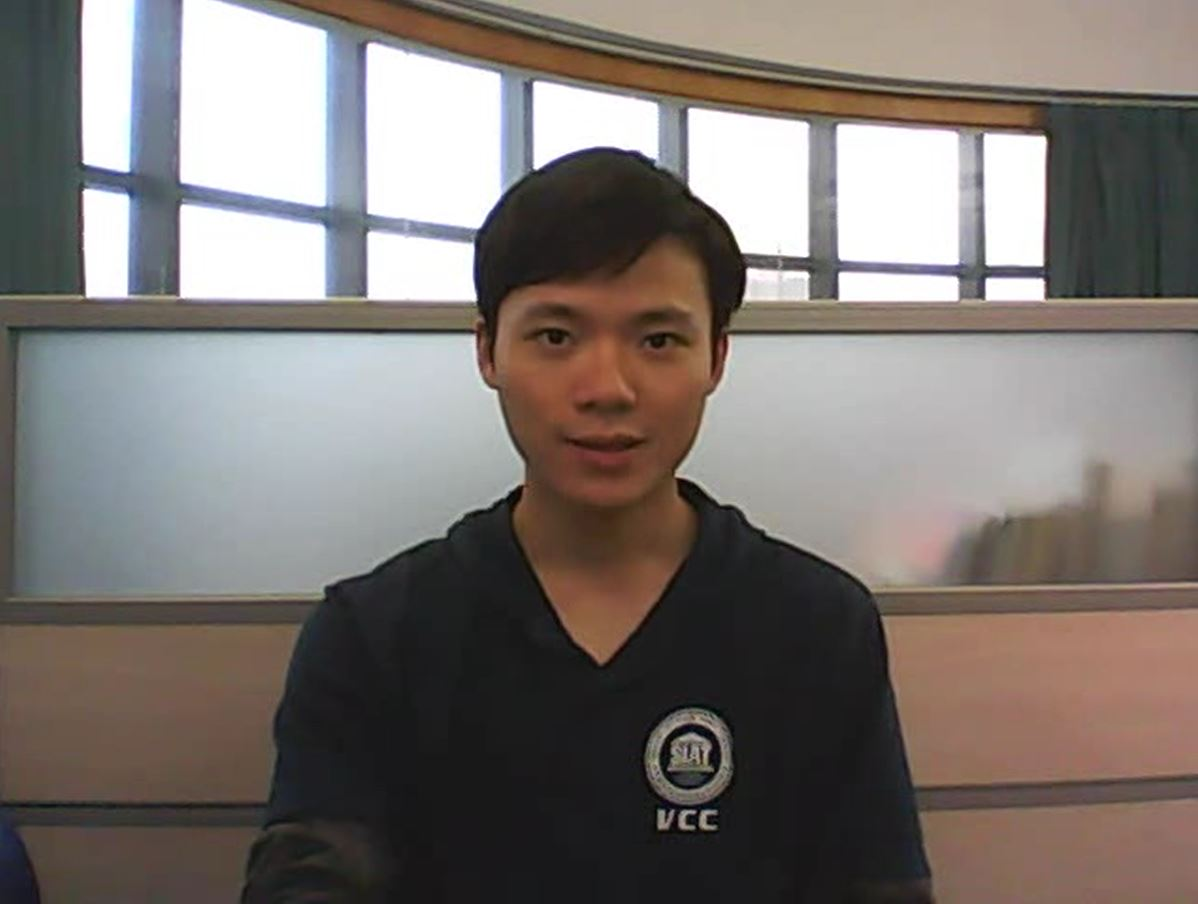
\includegraphics[height=23mm]{img/eulerian/test/man}
    \end{minipage}
      & 
    \begin{minipage}{.3\textwidth}
      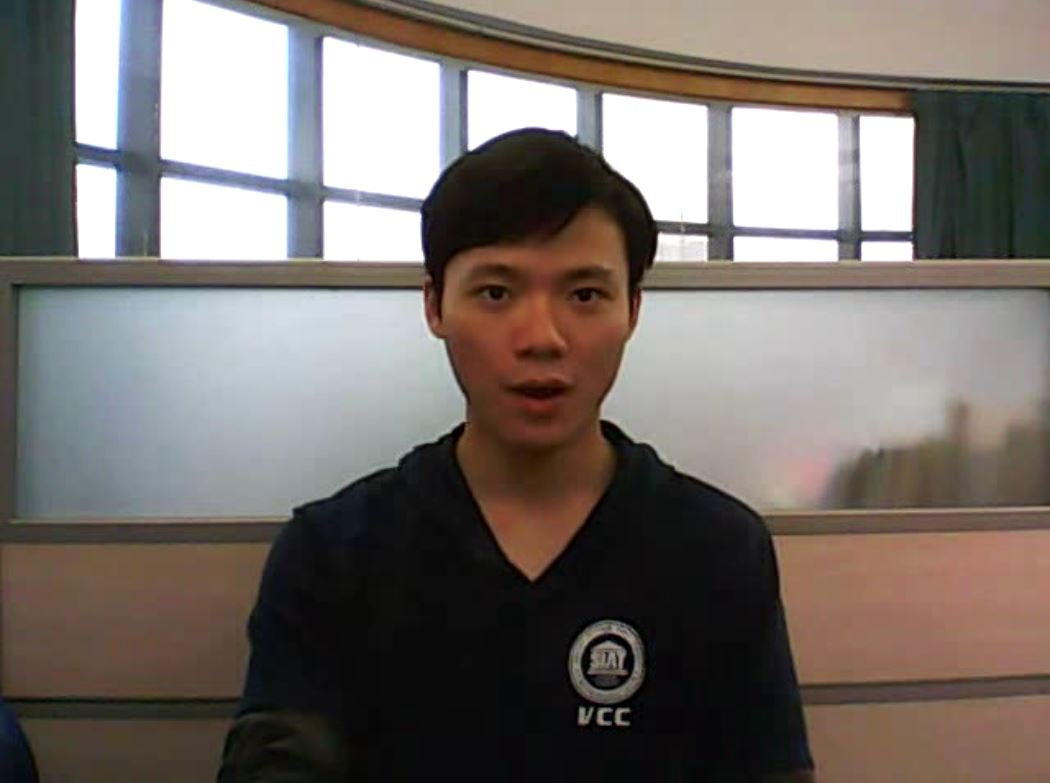
\includegraphics[height=23mm]{img/eulerian/test/mans}
    \end{minipage}
    \\
\hline
Man2 &85 & 30 & 0.85 & 1& \parbox[c]{1em}{
      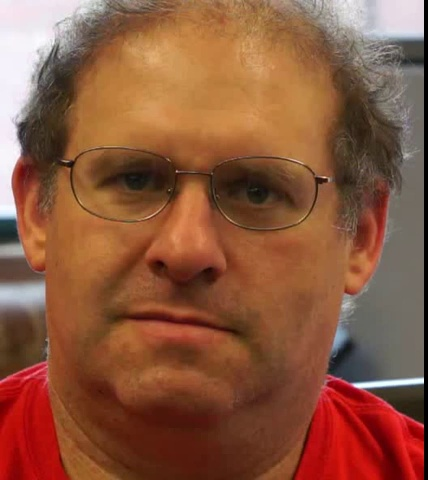
\includegraphics[height=23mm]{img/eulerian/test/man2}} & \parbox[c]{2em}{
      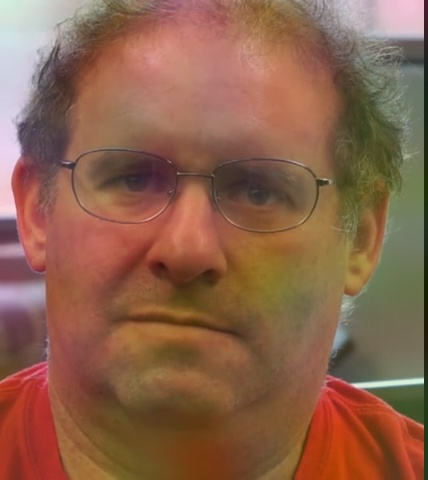
\includegraphics[height=23mm]{img/eulerian/test/man2s}} \\
\hline
Hand & 90 & 30 & 0.75 & 0.9 & \parbox[c]{1em}{
      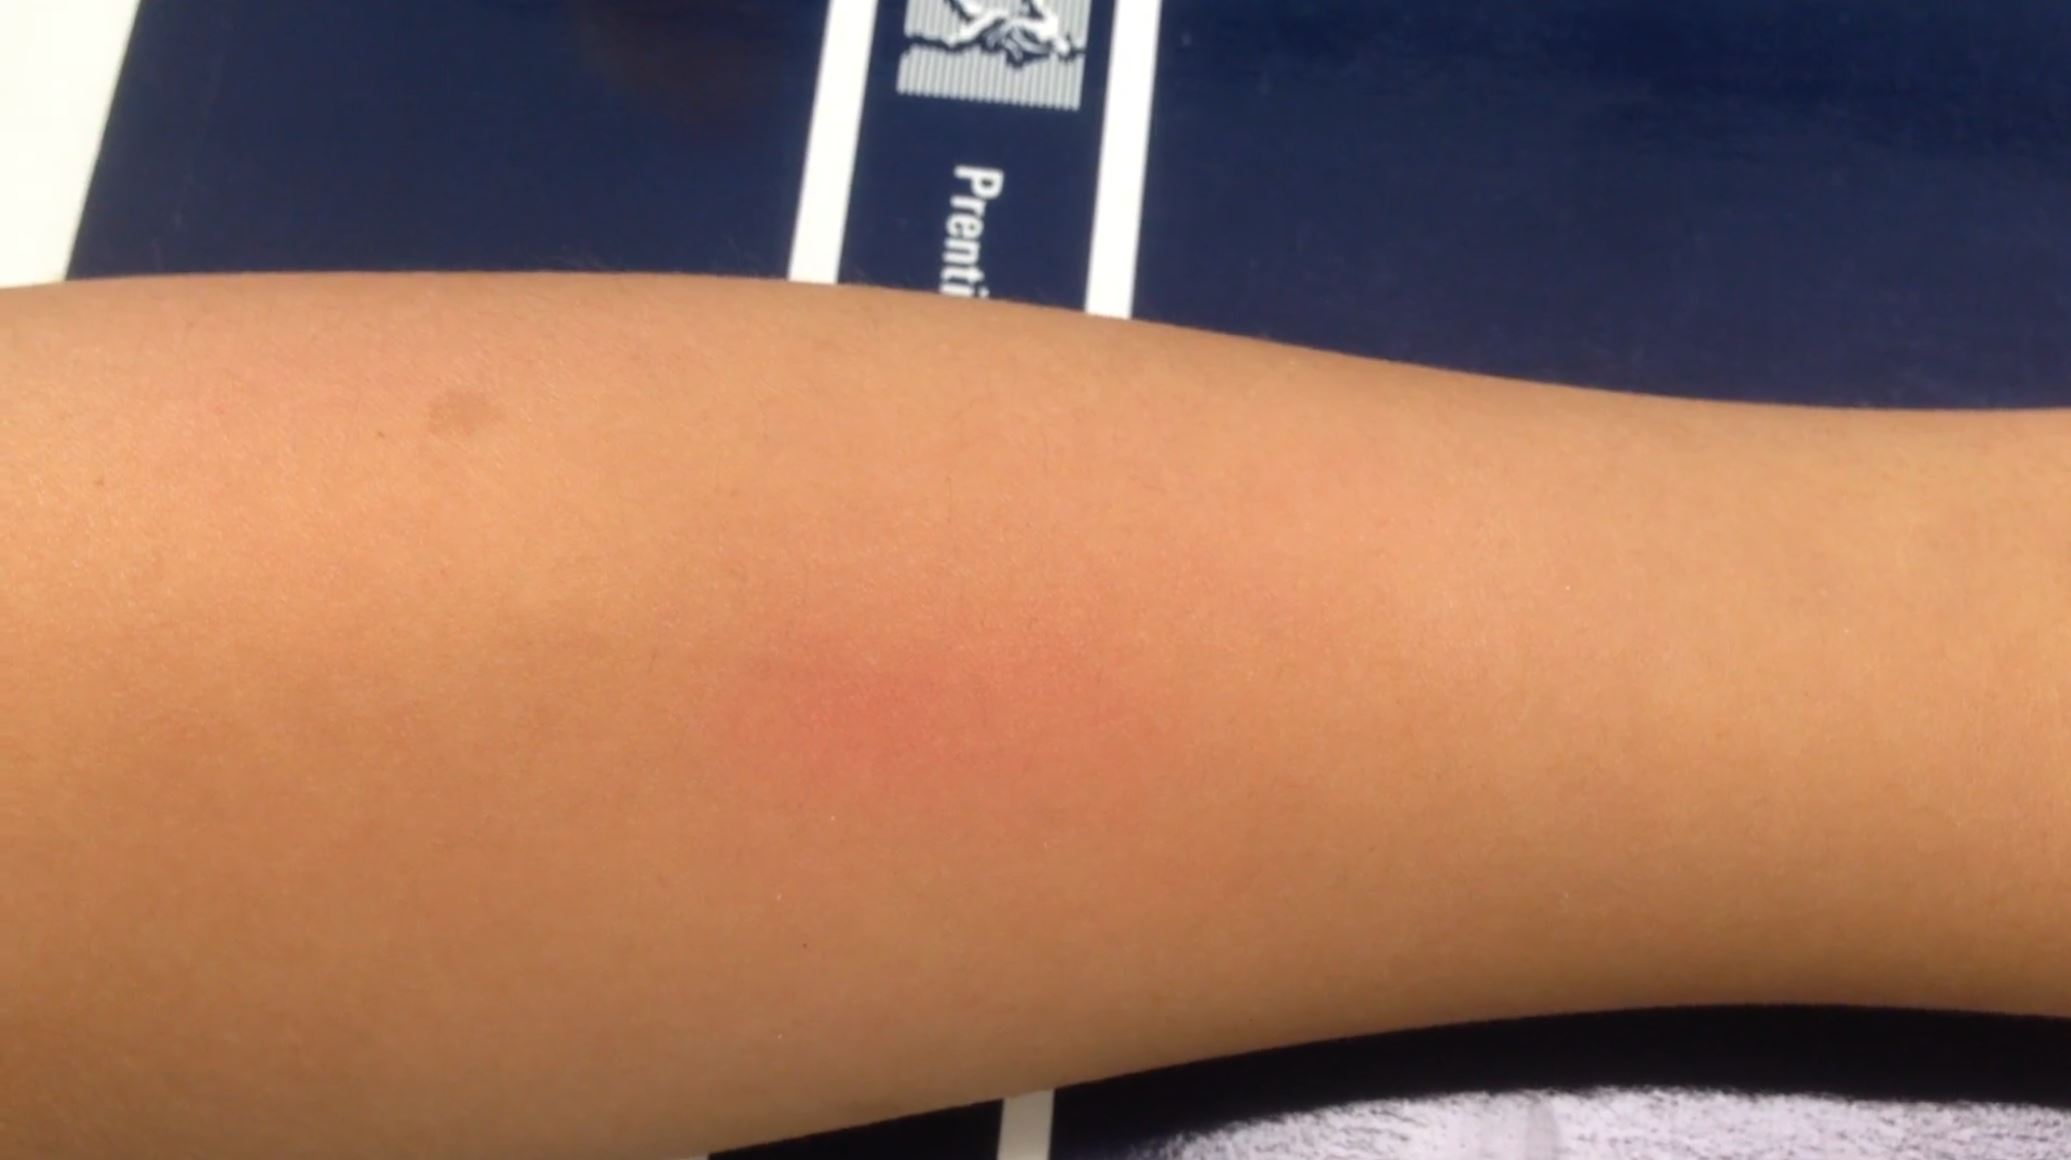
\includegraphics[height=20mm]{img/eulerian/test/hand}} & \parbox[c]{1em}{
      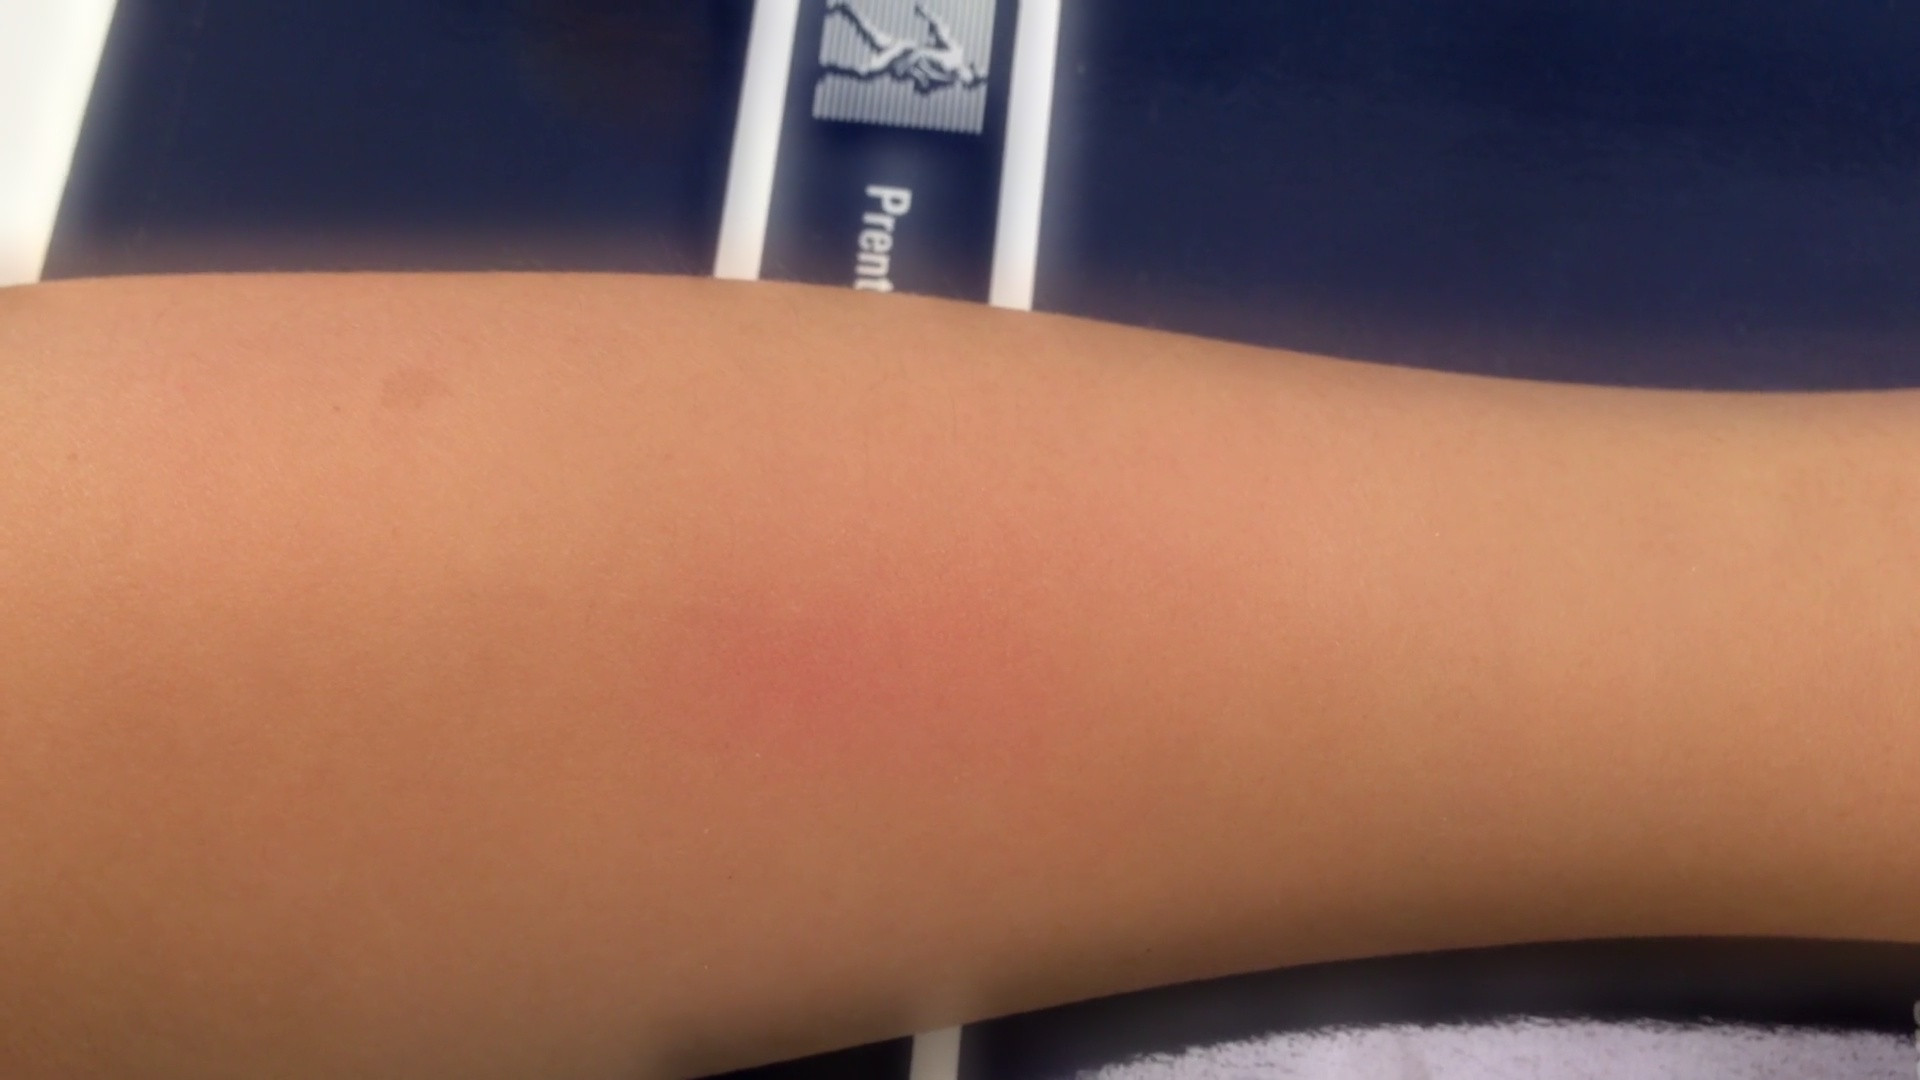
\includegraphics[height=20mm]{img/eulerian/sample/120}} \\
\hline
Hand2 & 90 & 30 & 0.75 &  0.9 & \parbox[c]{1em}{
      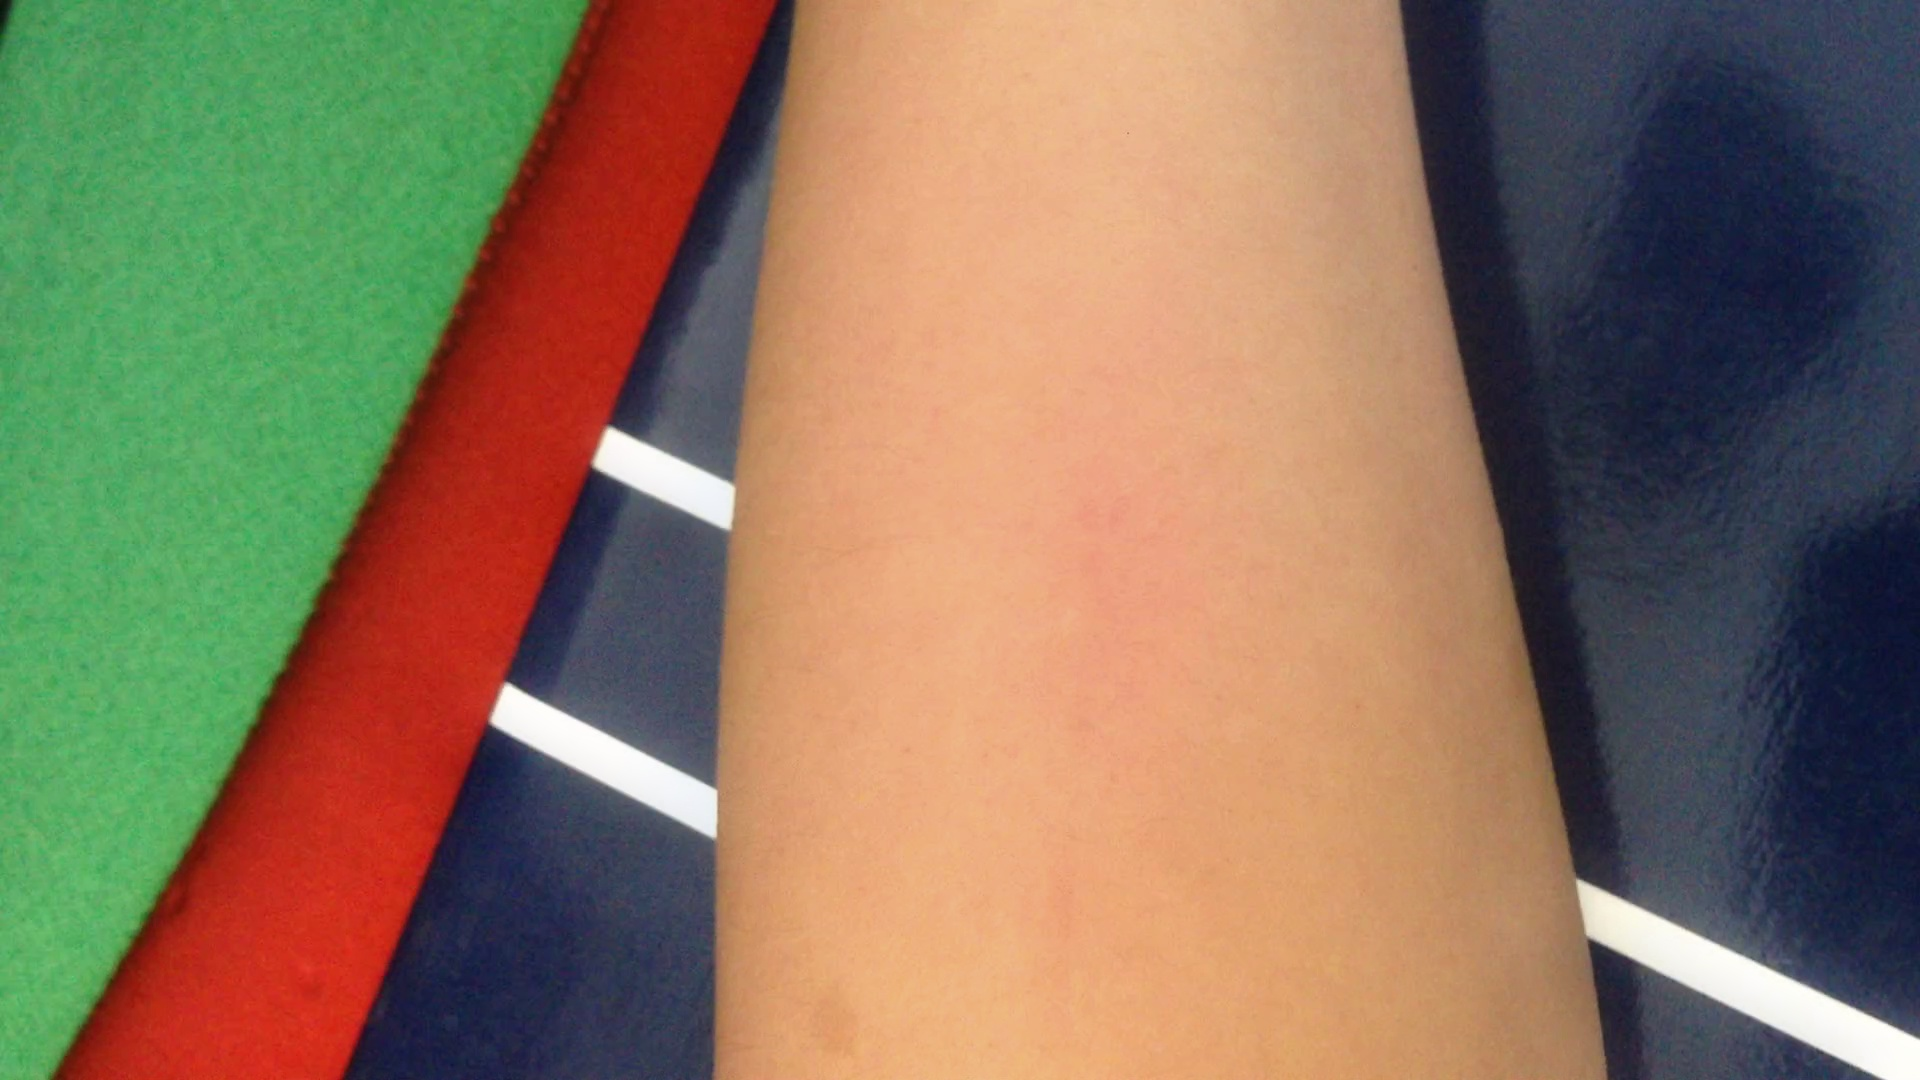
\includegraphics[height=20mm]{img/eulerian/test/hand2}} & 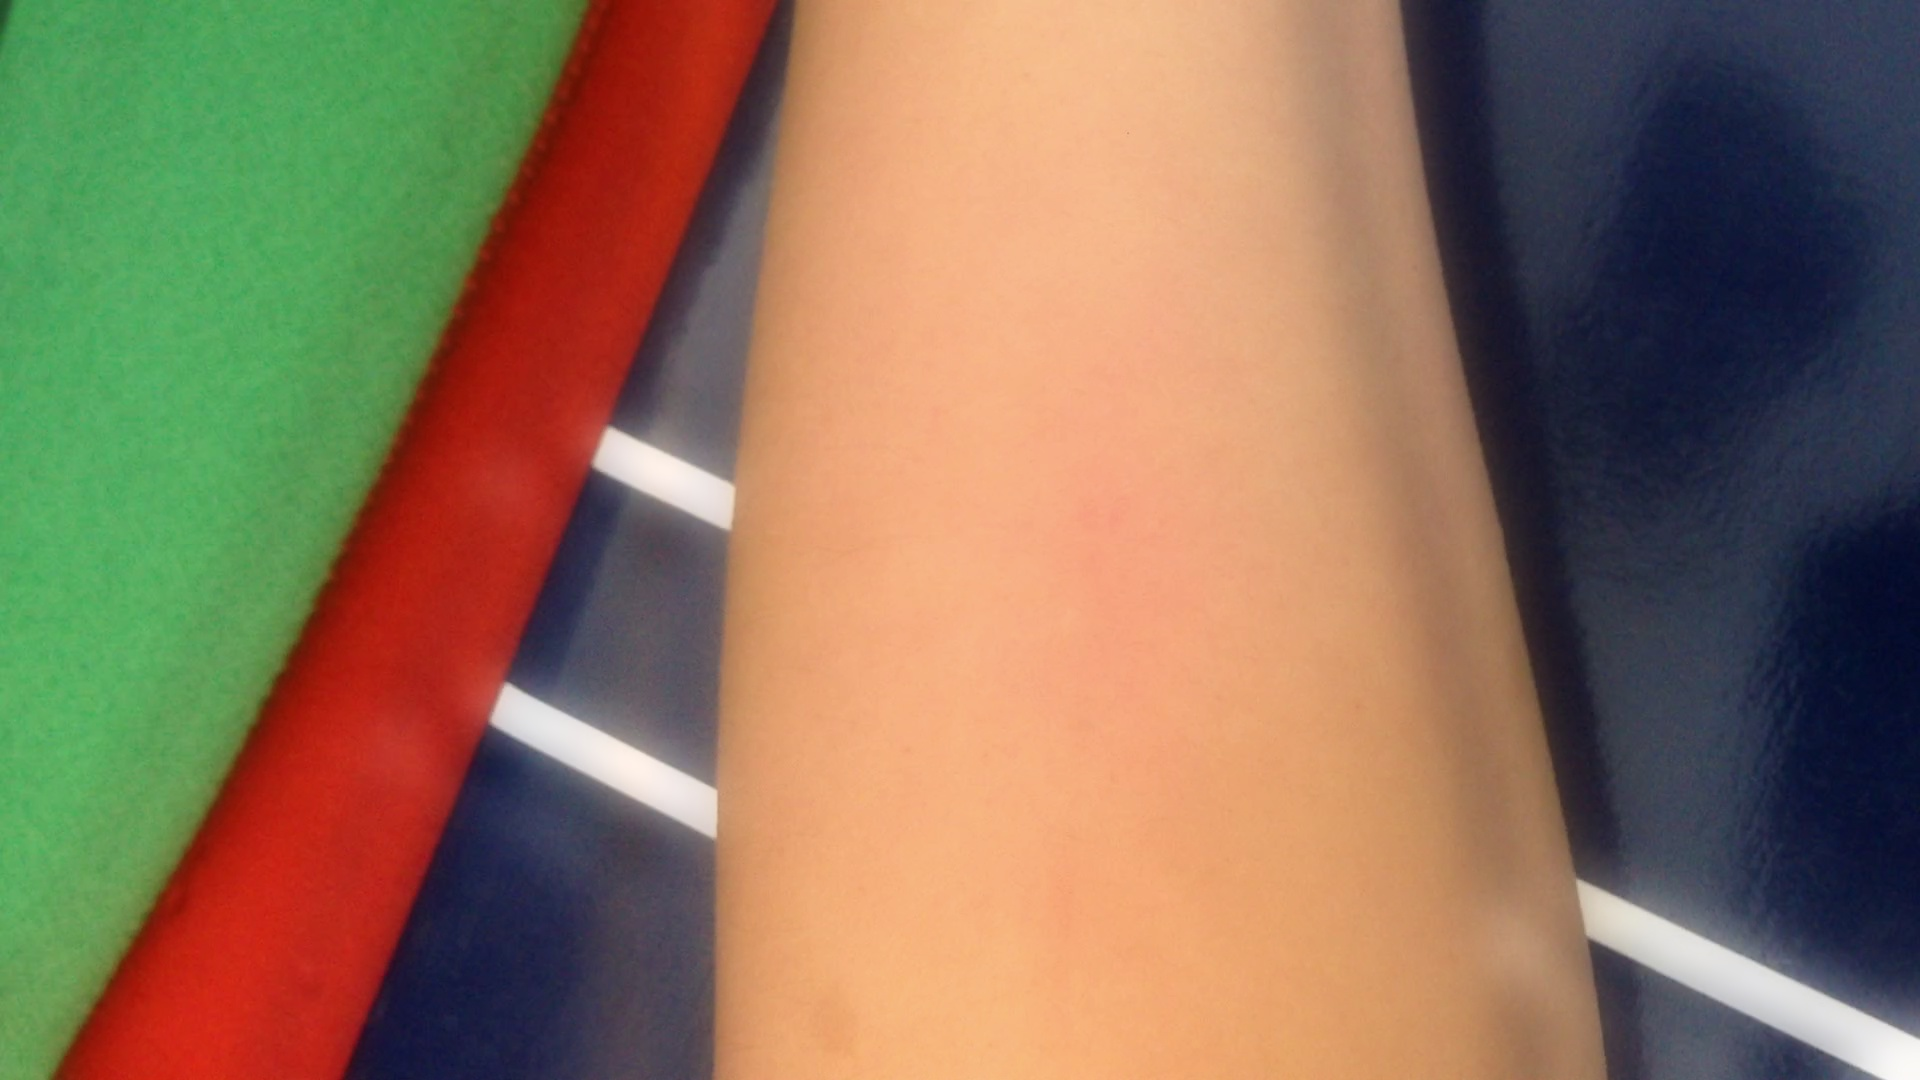
\includegraphics[height=20mm]{img/eulerian/test/hand2s} \\ 
\hline
Leg & 90 & 30 & 0.8 & 0.95  & 
      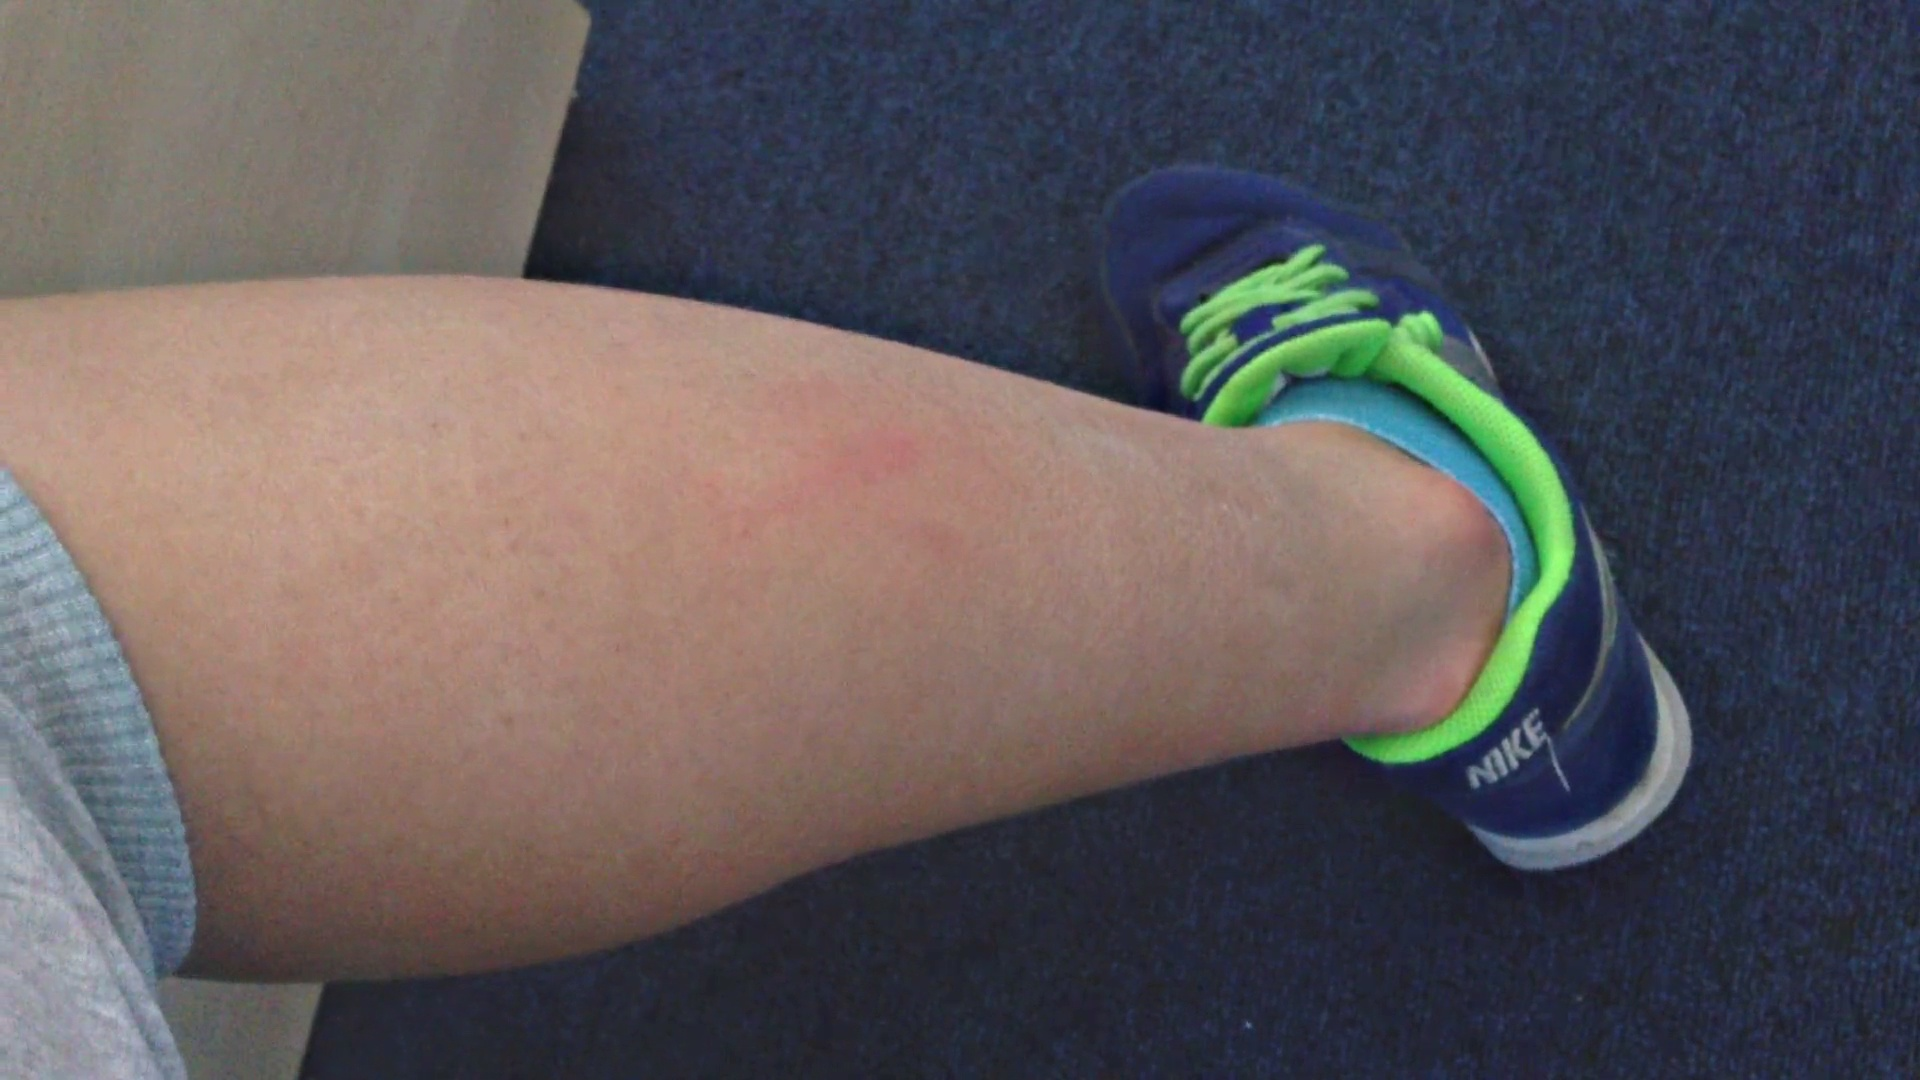
\includegraphics[height=20mm]{img/eulerian/test/leg} & 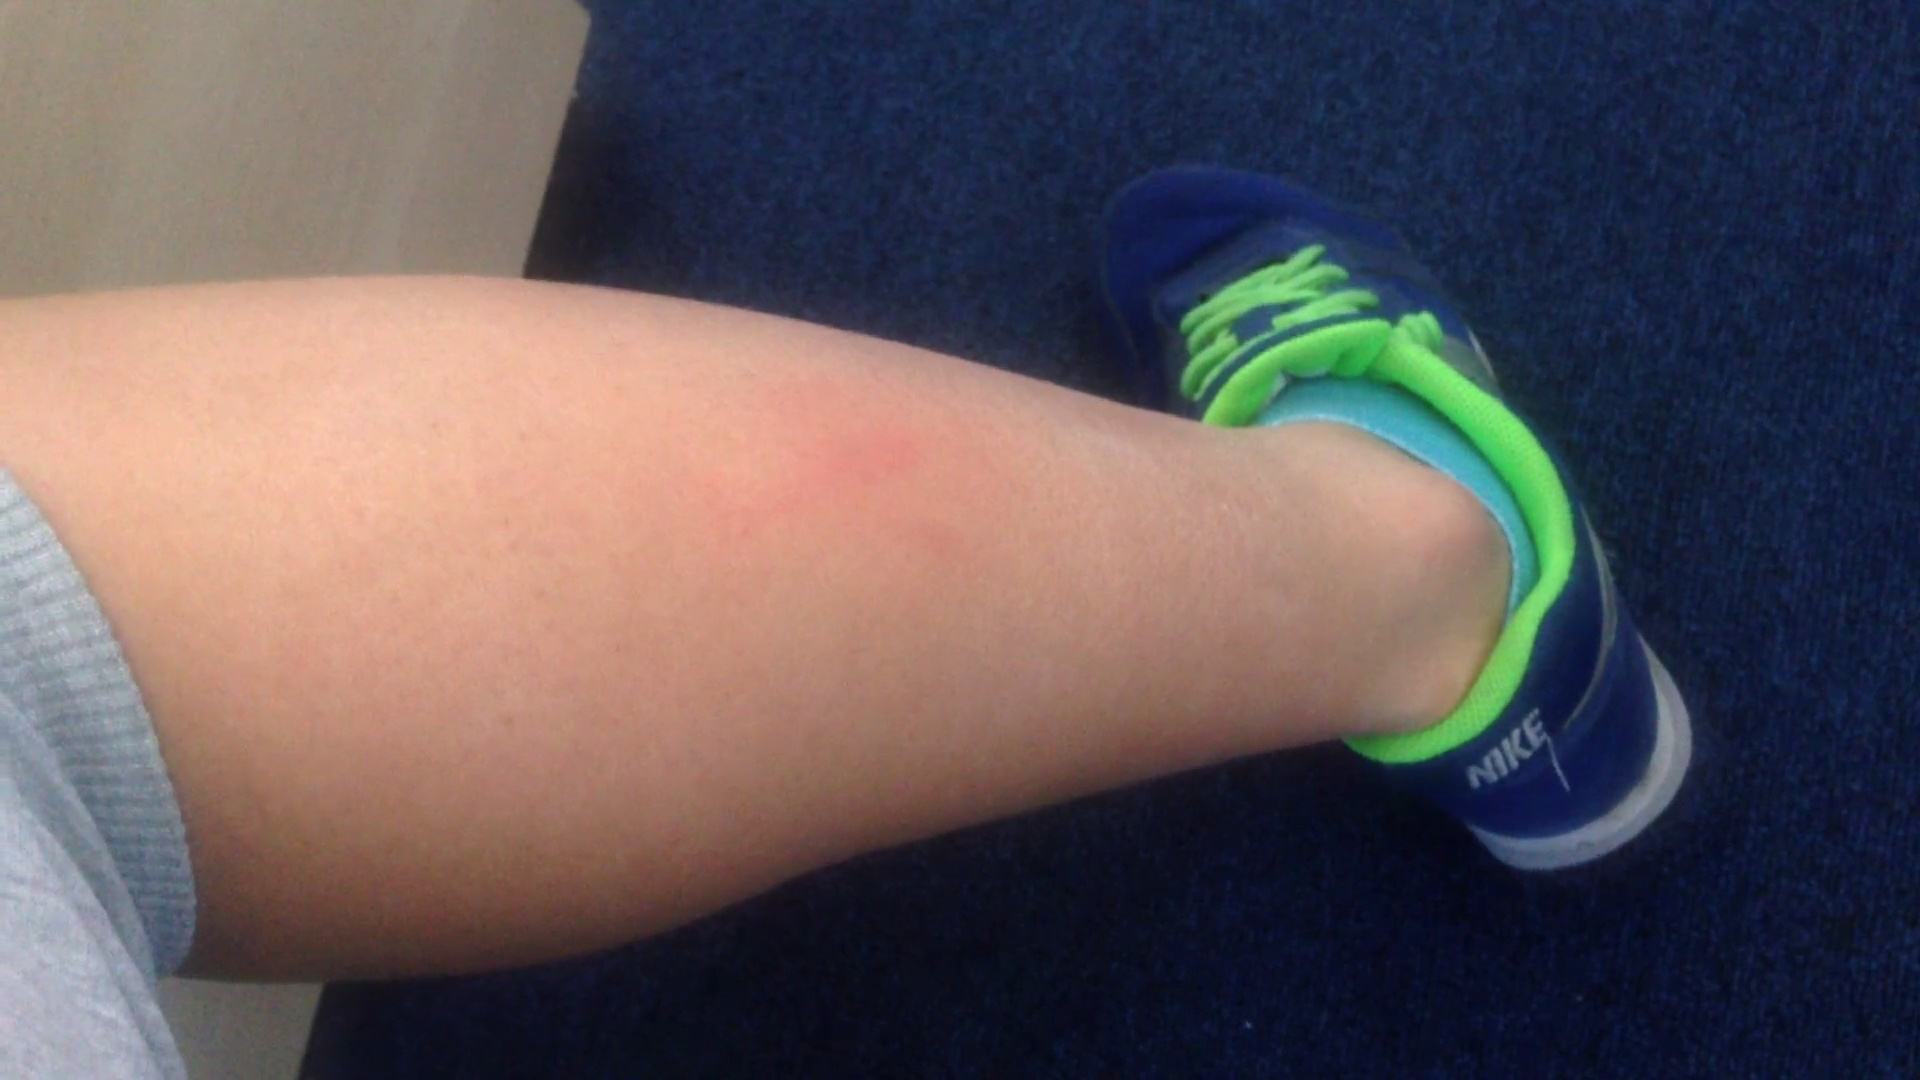
\includegraphics[height=20mm]{img/eulerian/test/legs}\\
\hline
Leg2 & 90 & 30 & 0.8 & 0.95 & \parbox[c]{1em}{
      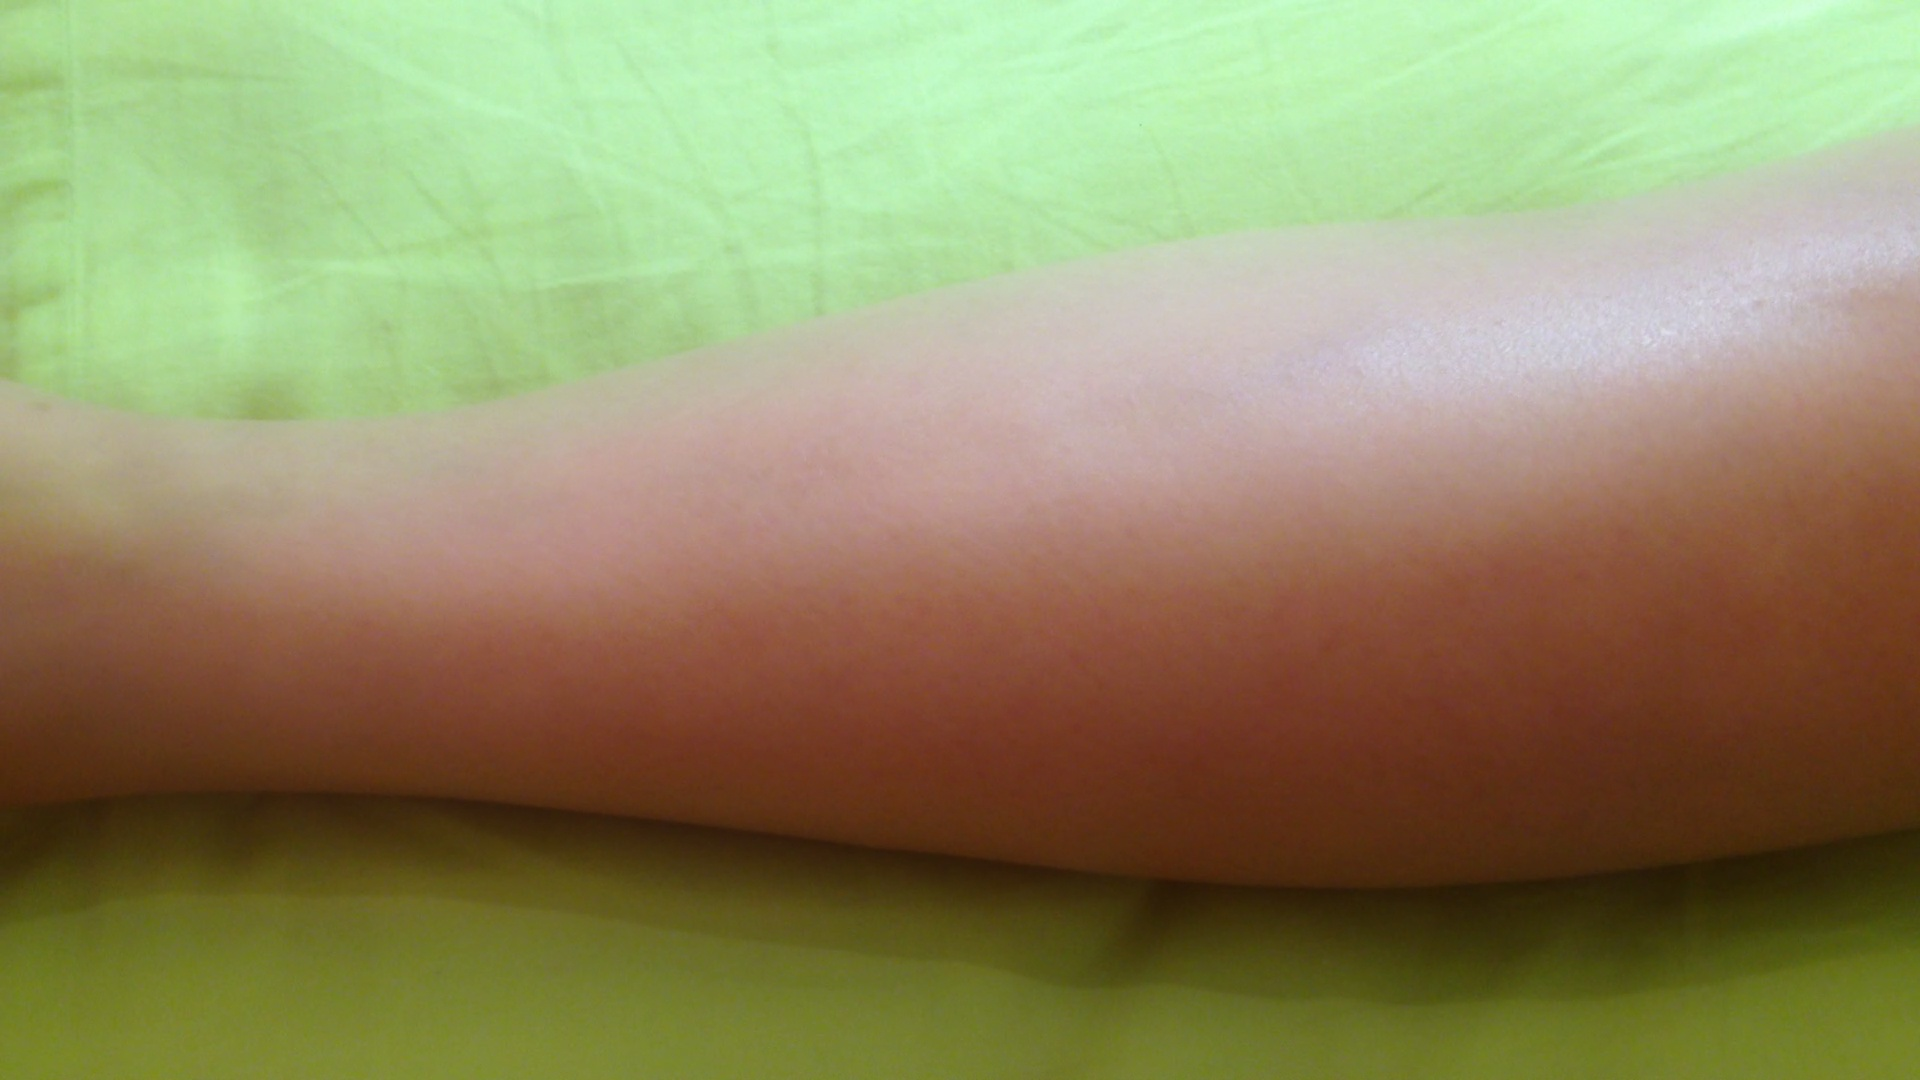
\includegraphics[height=20mm]{img/eulerian/test/leg2}} & \parbox[c]{1em}{
      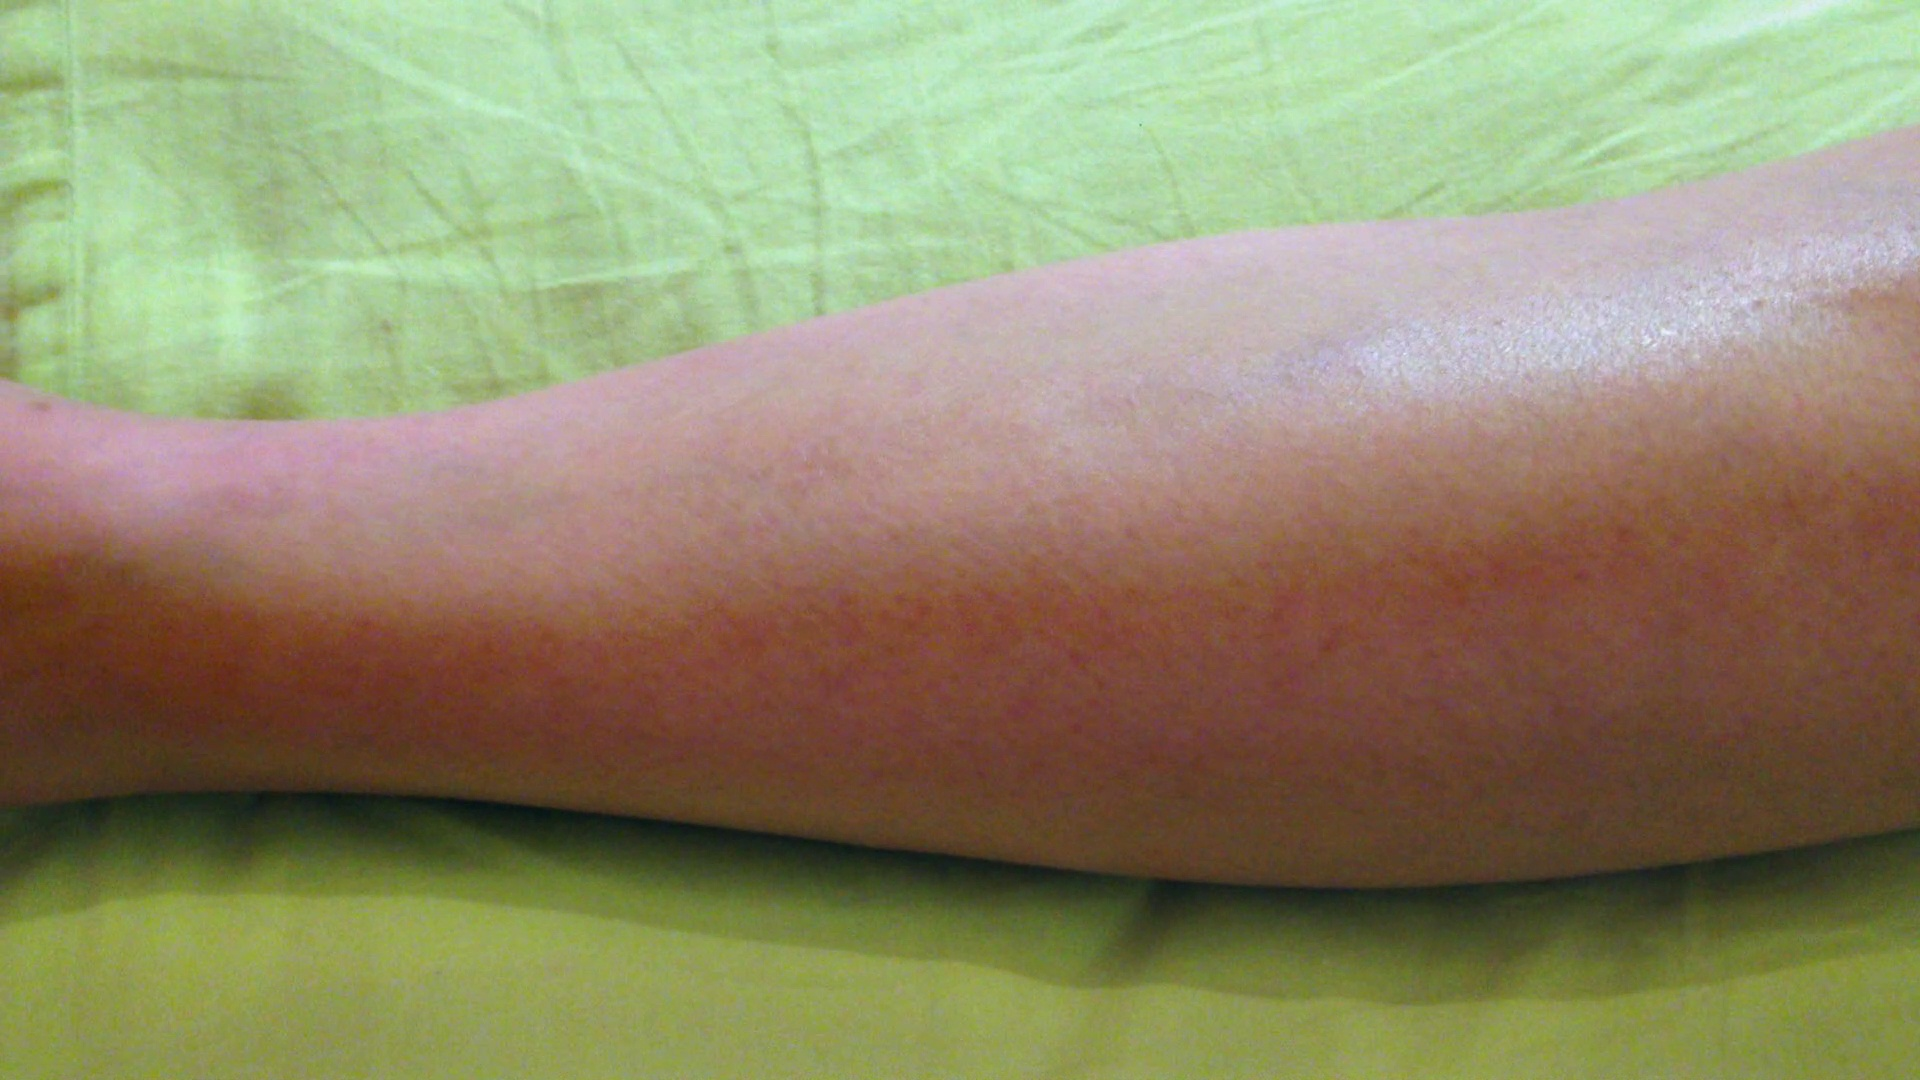
\includegraphics[height=20mm]{img/eulerian/test/leg2s}} \\ 
\hline
\end{tabular}
\begin{tablenotes}
        \footnotesize
        \item[1] $\alpha$: amplification factor
        \item[2] $\lambda$: frame rate
        \item[3] $f_{l}$: frequency lower
        \item[4] $f_{h}$: frequency upper
\end{tablenotes}
\end{threeparttable}
\end{table}

\section{Experimental Result Analysis}
The first two experiments using the darker face, and another one with lighter complexion is from the the homepage of Eulerian Video Magnification Research Group. In both videos, the objectives were to amplify
the color change as the blood flows through the face. Apply gaussian pyramid for the level 5. For each video, passed each sequence of frames through the ideal bandpass filter with a passband of 0.85 Hz to 1 Hz (50 bpm to 60 bpm). Finally, a large value of $\alpha = 85$ and $\lambda =30$ was
applied to the resulting spatially lowpass signal to emphasize the color changes as much as possible. The final video was formed by adding the signal back to the original.\\

For man2 face changes are very clear after Eulerian Video Magnification from 1 second to 3 second, specailly his forehead. Although the background is color-magnified also. For man face, the changes are not so obvious as the man2,  which was exposed to a strong controlled backlight in order to make the vein structure partly visible in the recorded video. The magnified video did not reveal any observable patterns that would suggest that the pulse was visualized. The periodic pattern in the magnified video exhibited the same properties as in the previous experiment, suggesting that it is caused by the slight movements of the hand held still.\\

In the next experiment, the hands (or any area with the pressure ulcers) are very difficult to find the correct frequency range. The both (hand and hand2) changes affects after Eulerian Video Magnification are not so obvious. And in the second hand, move a bit during the video to check the influences of movement on this algorithms.\\

\begin{figure}[!h]
\centering
\begin{subfigure}{.3\textwidth}
  \centering
  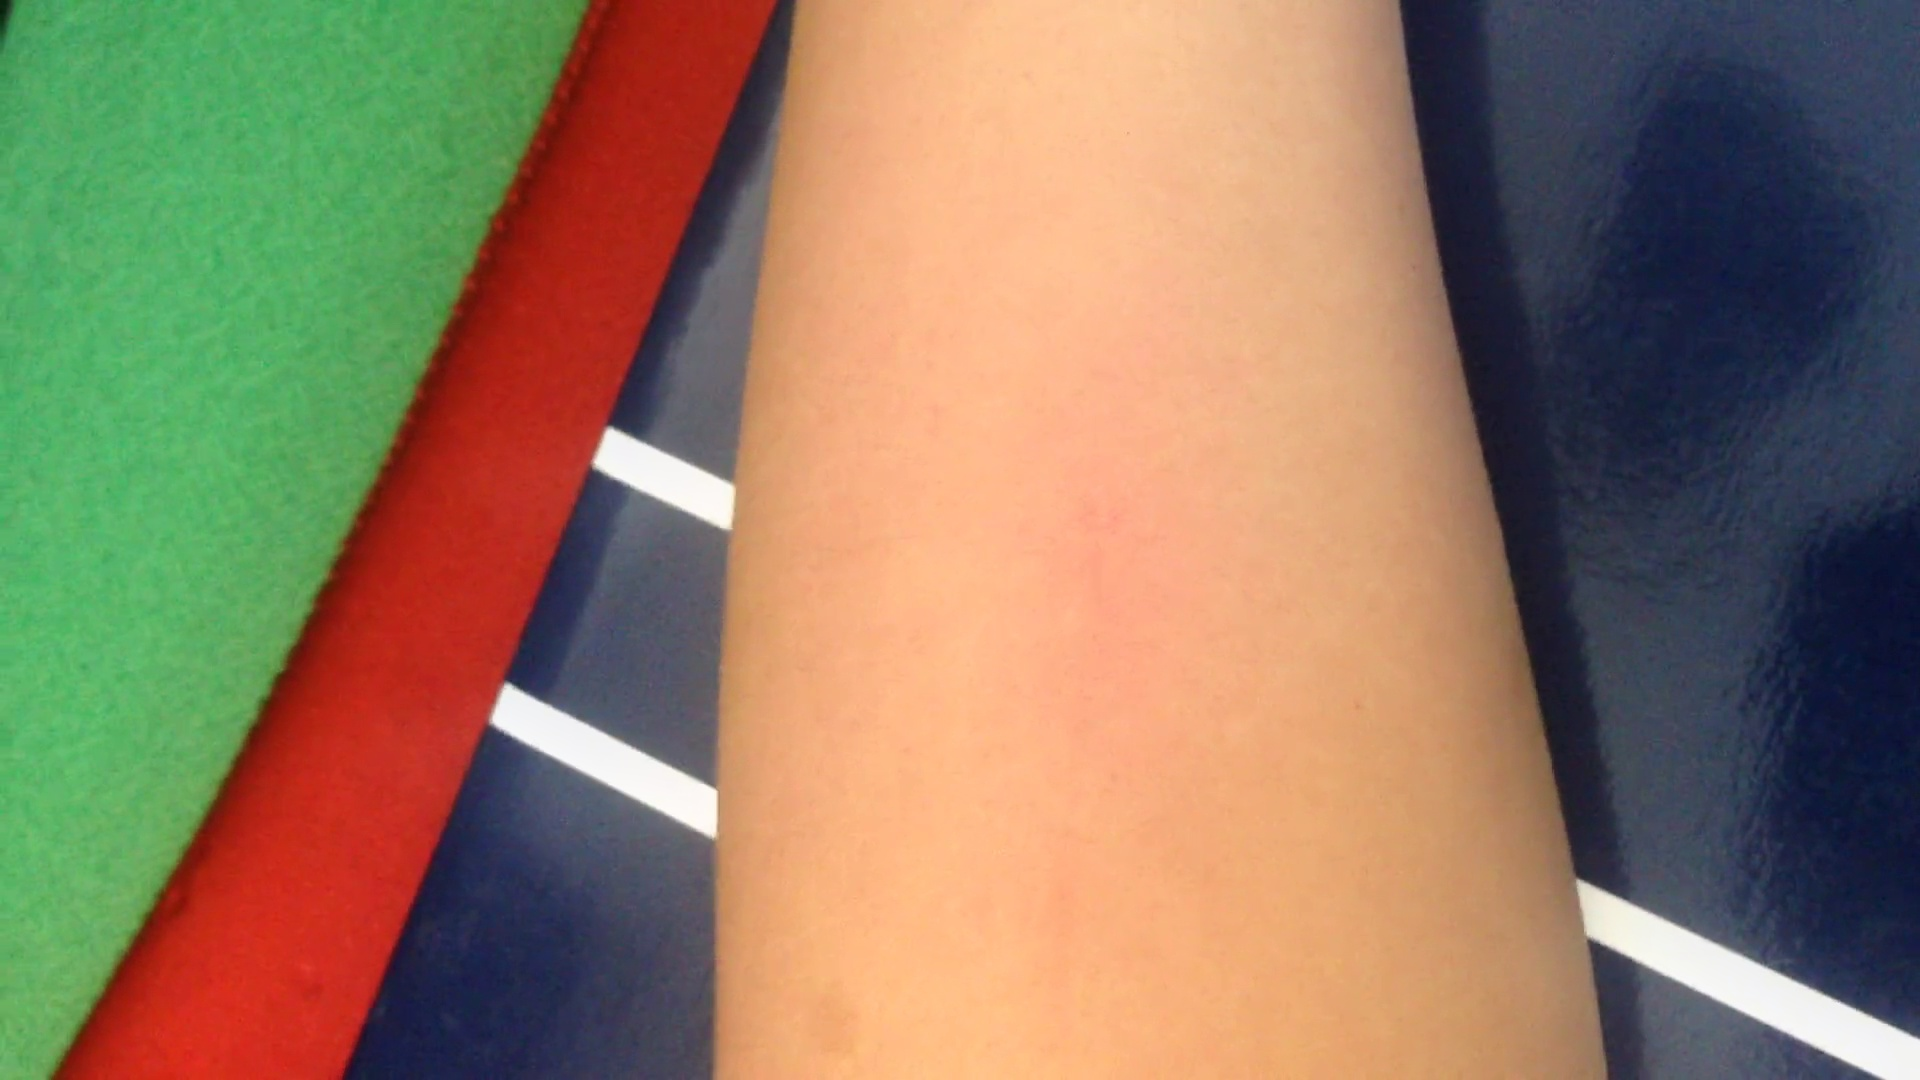
\includegraphics[scale=0.08]{img/eulerian/test/handc1}
  \label{fig:sub2}
\end{subfigure}%
\begin{subfigure}{.3\textwidth}
  \centering
  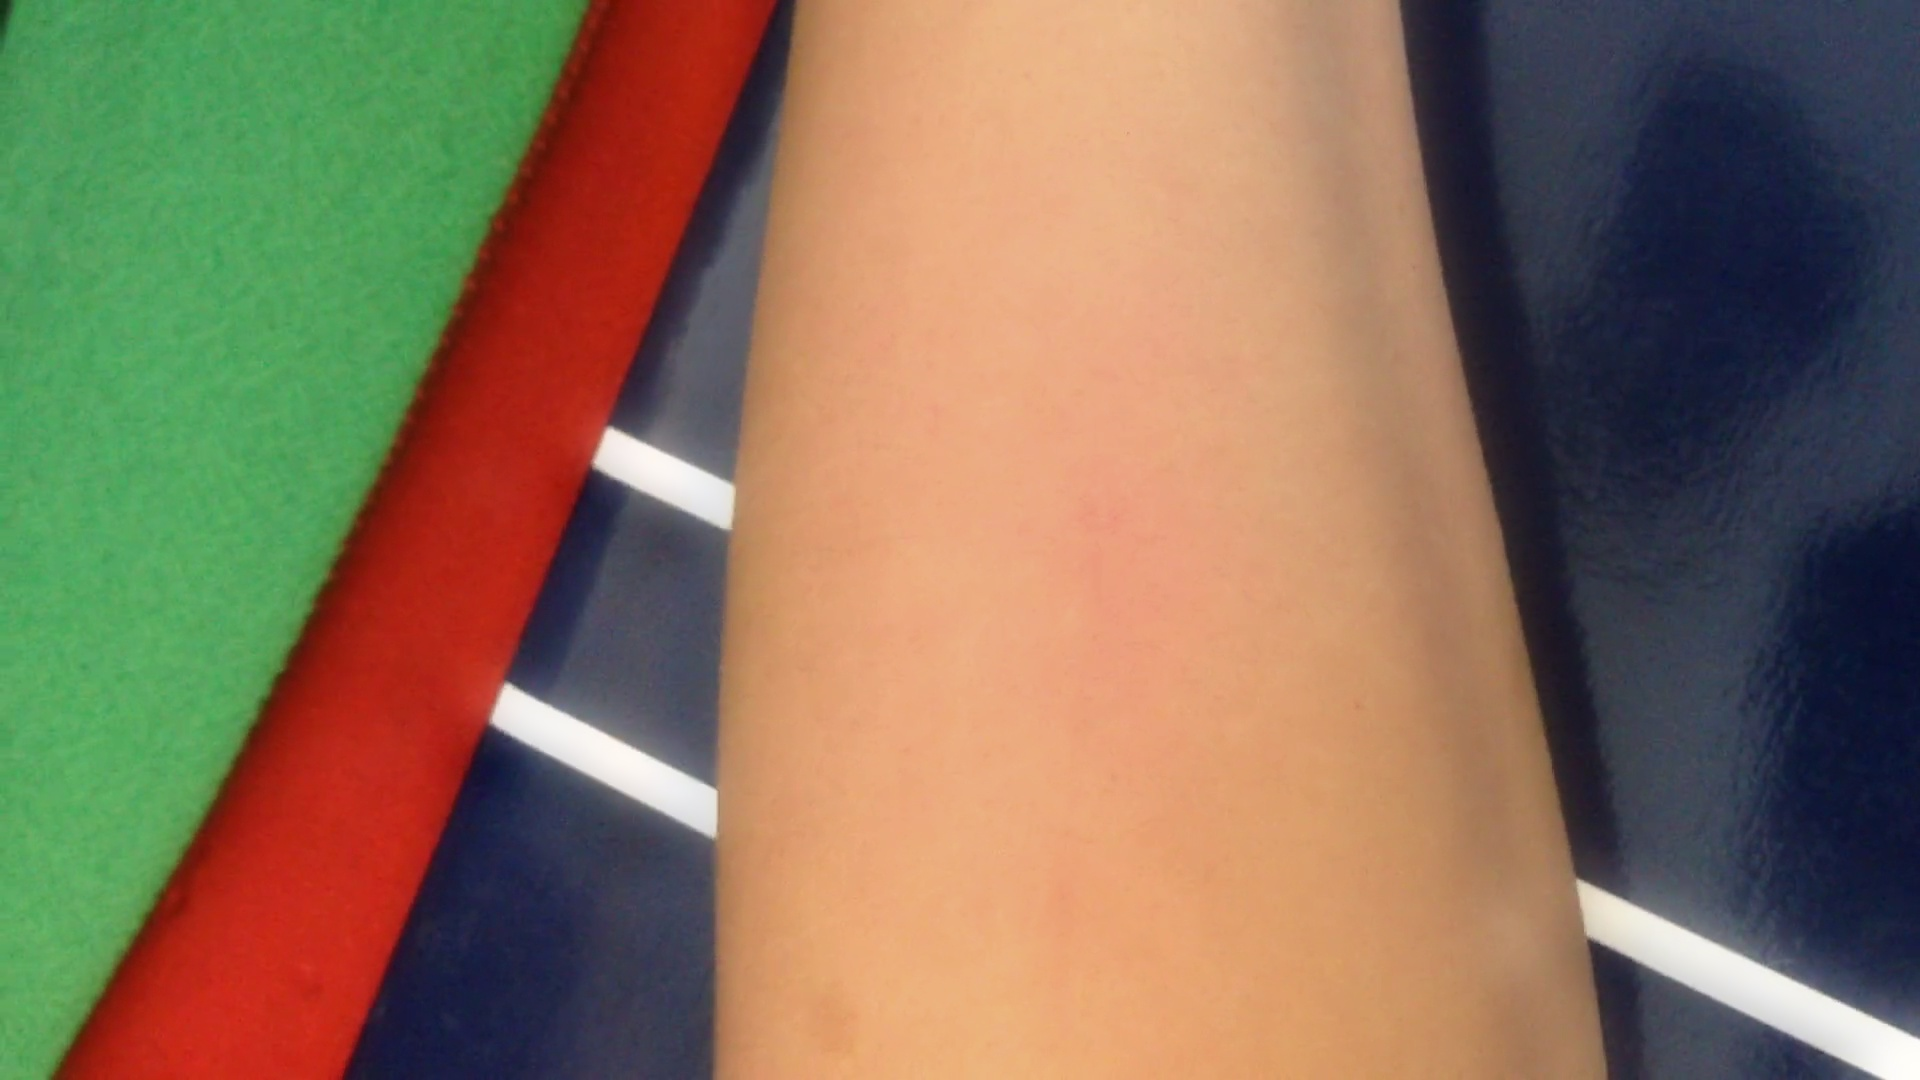
\includegraphics[scale=0.08]{img/eulerian/test/handc2}
  \label{fig:sub2}
\end{subfigure}
\begin{subfigure}{.3\textwidth}
  \centering
  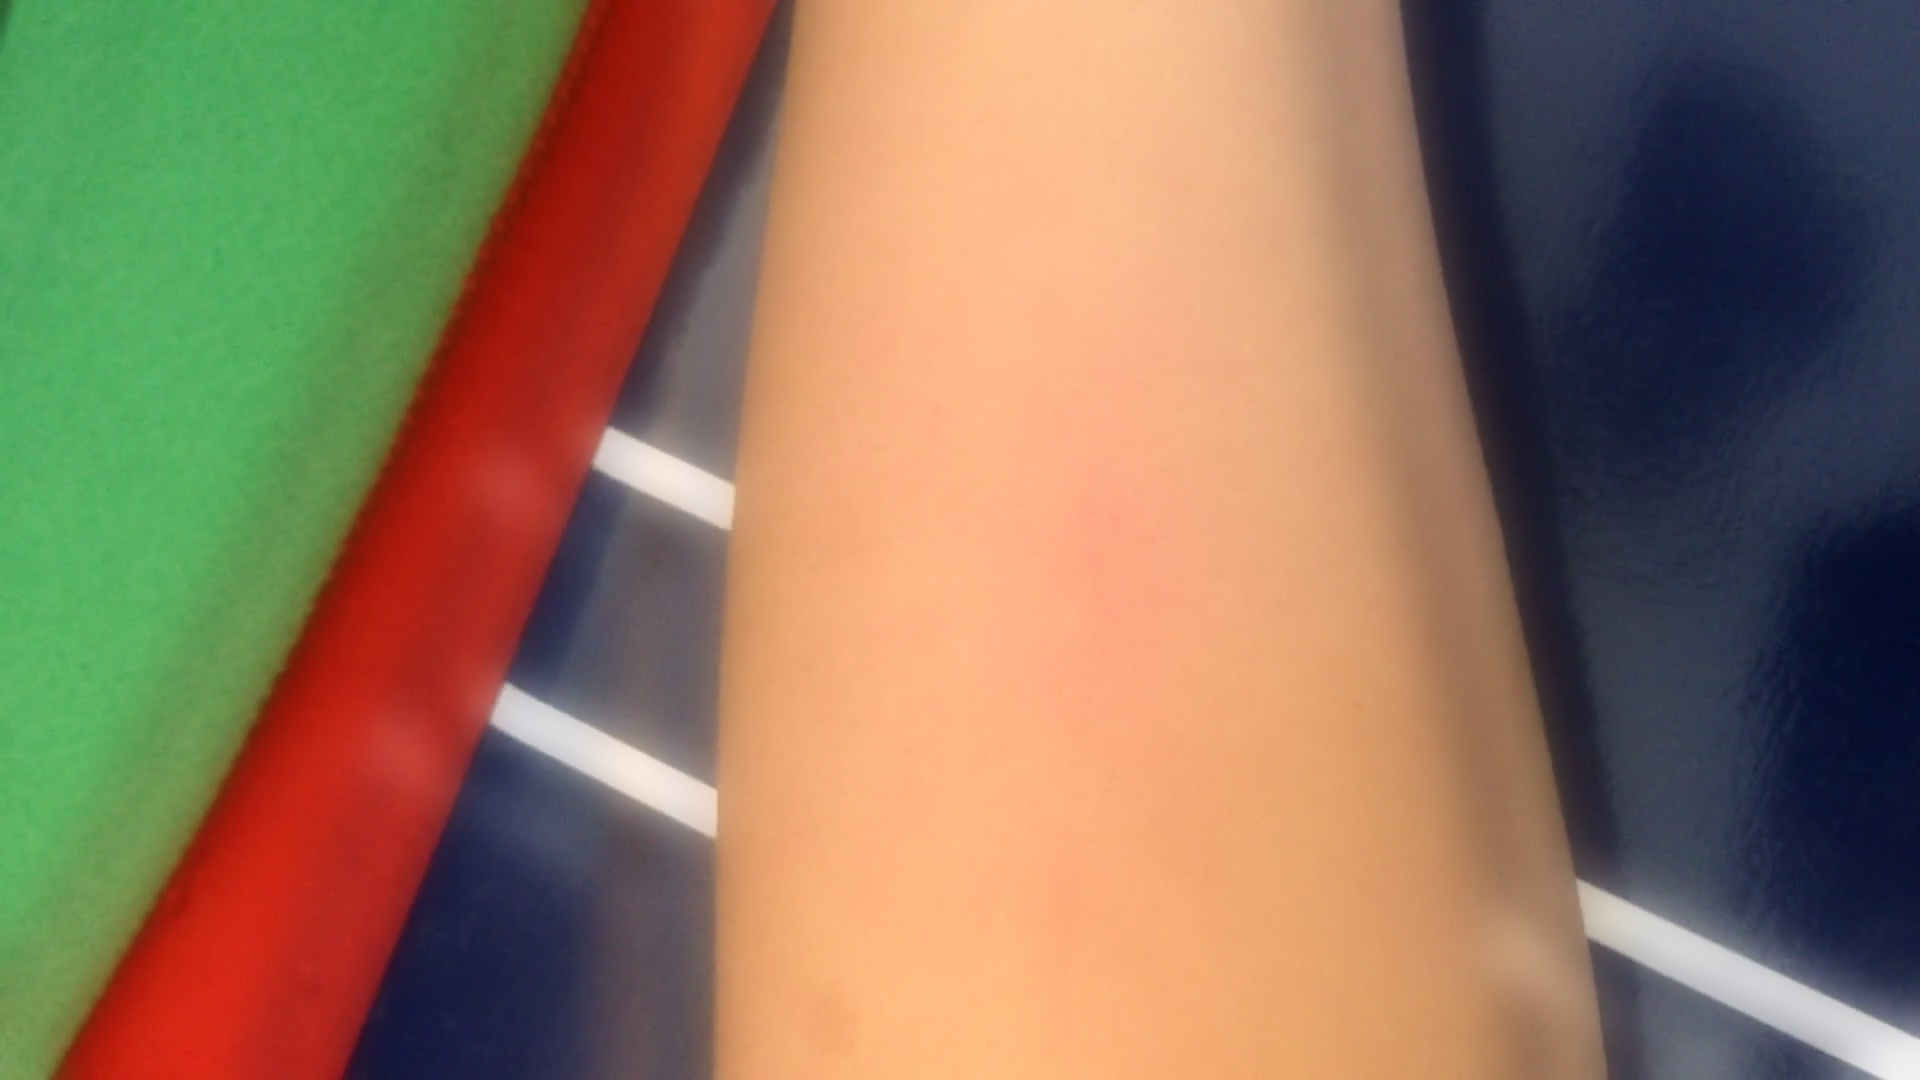
\includegraphics[scale=0.08]{img/eulerian/test/handc3}
  \label{fig:sub2}
\end{subfigure}
\begin{subfigure}{.3\textwidth}
  \centering
  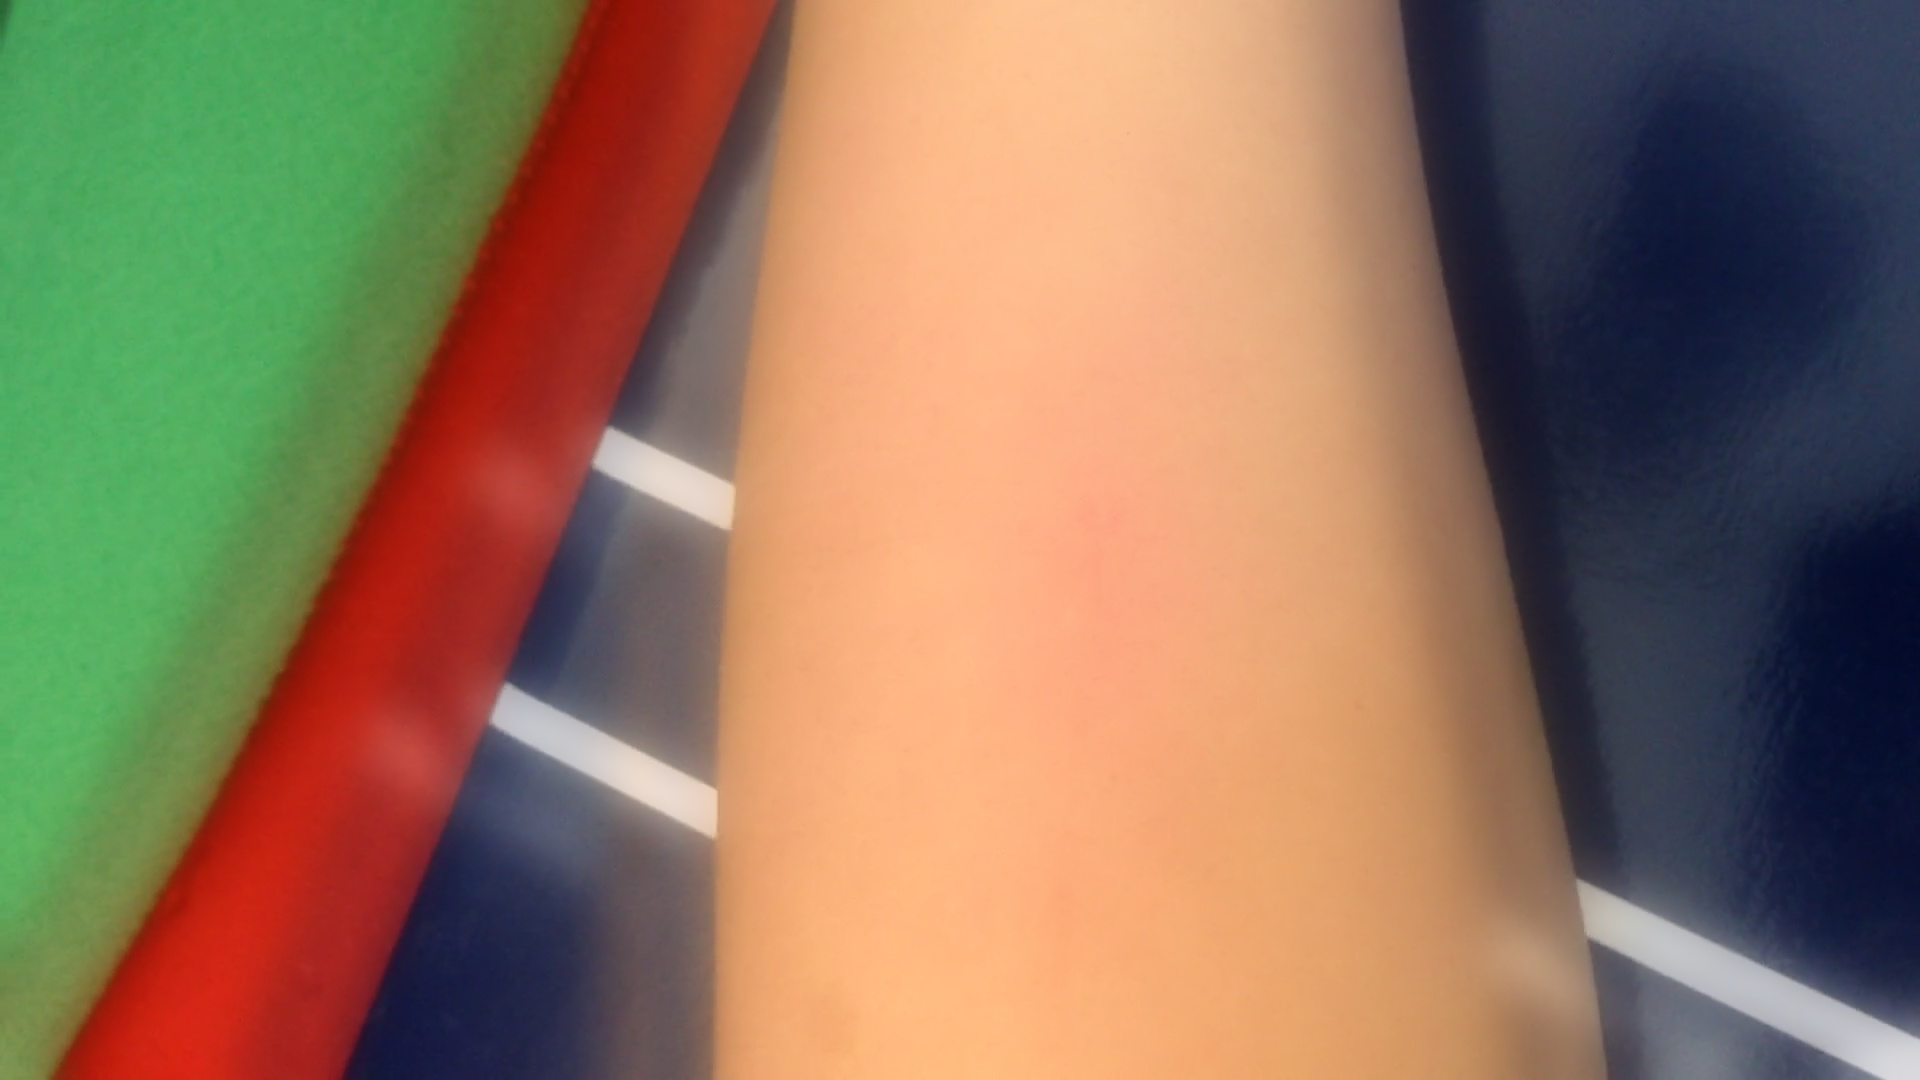
\includegraphics[scale=0.08]{img/eulerian/test/handc4}
  \label{fig:sub2}
\end{subfigure}%
\begin{subfigure}{.3\textwidth}
  \centering
  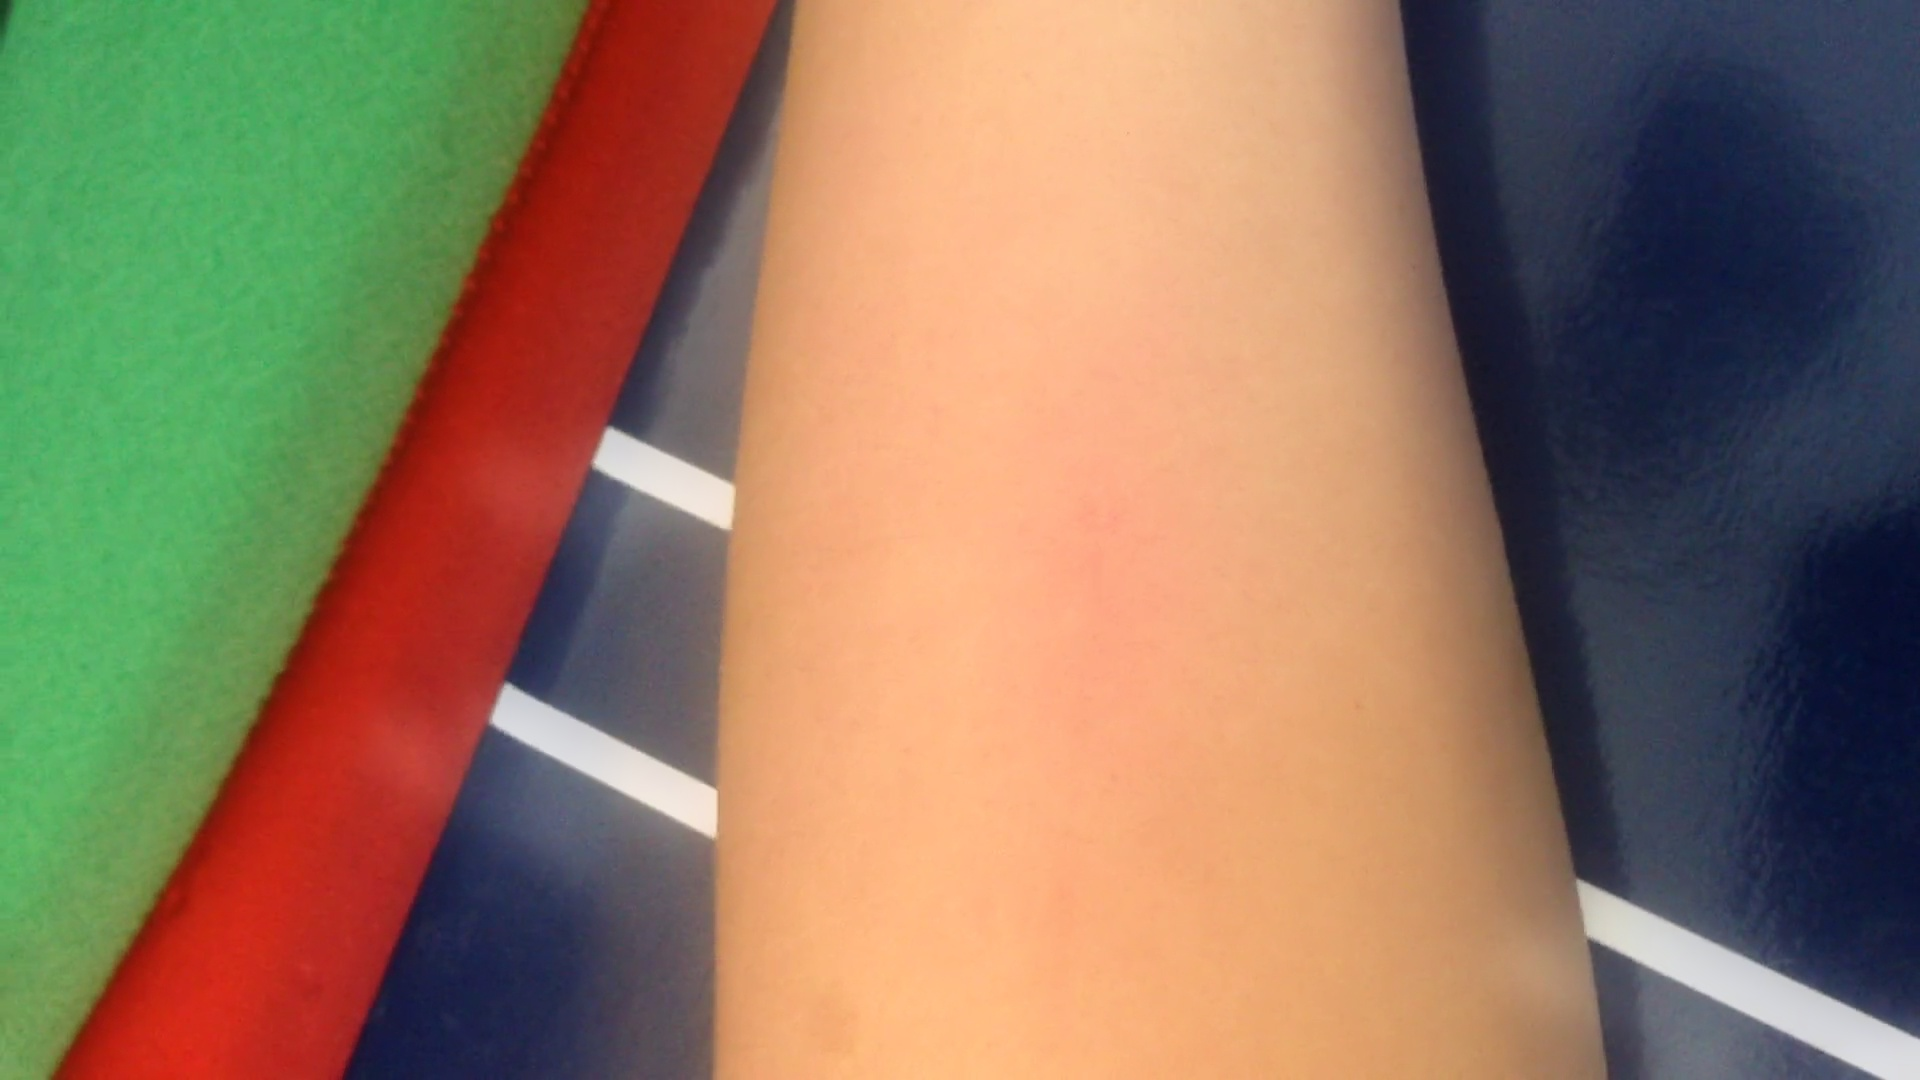
\includegraphics[scale=0.08]{img/eulerian/test/handc5}
  \label{fig:sub2}
\end{subfigure}
\begin{subfigure}{.3\textwidth}
  \centering
  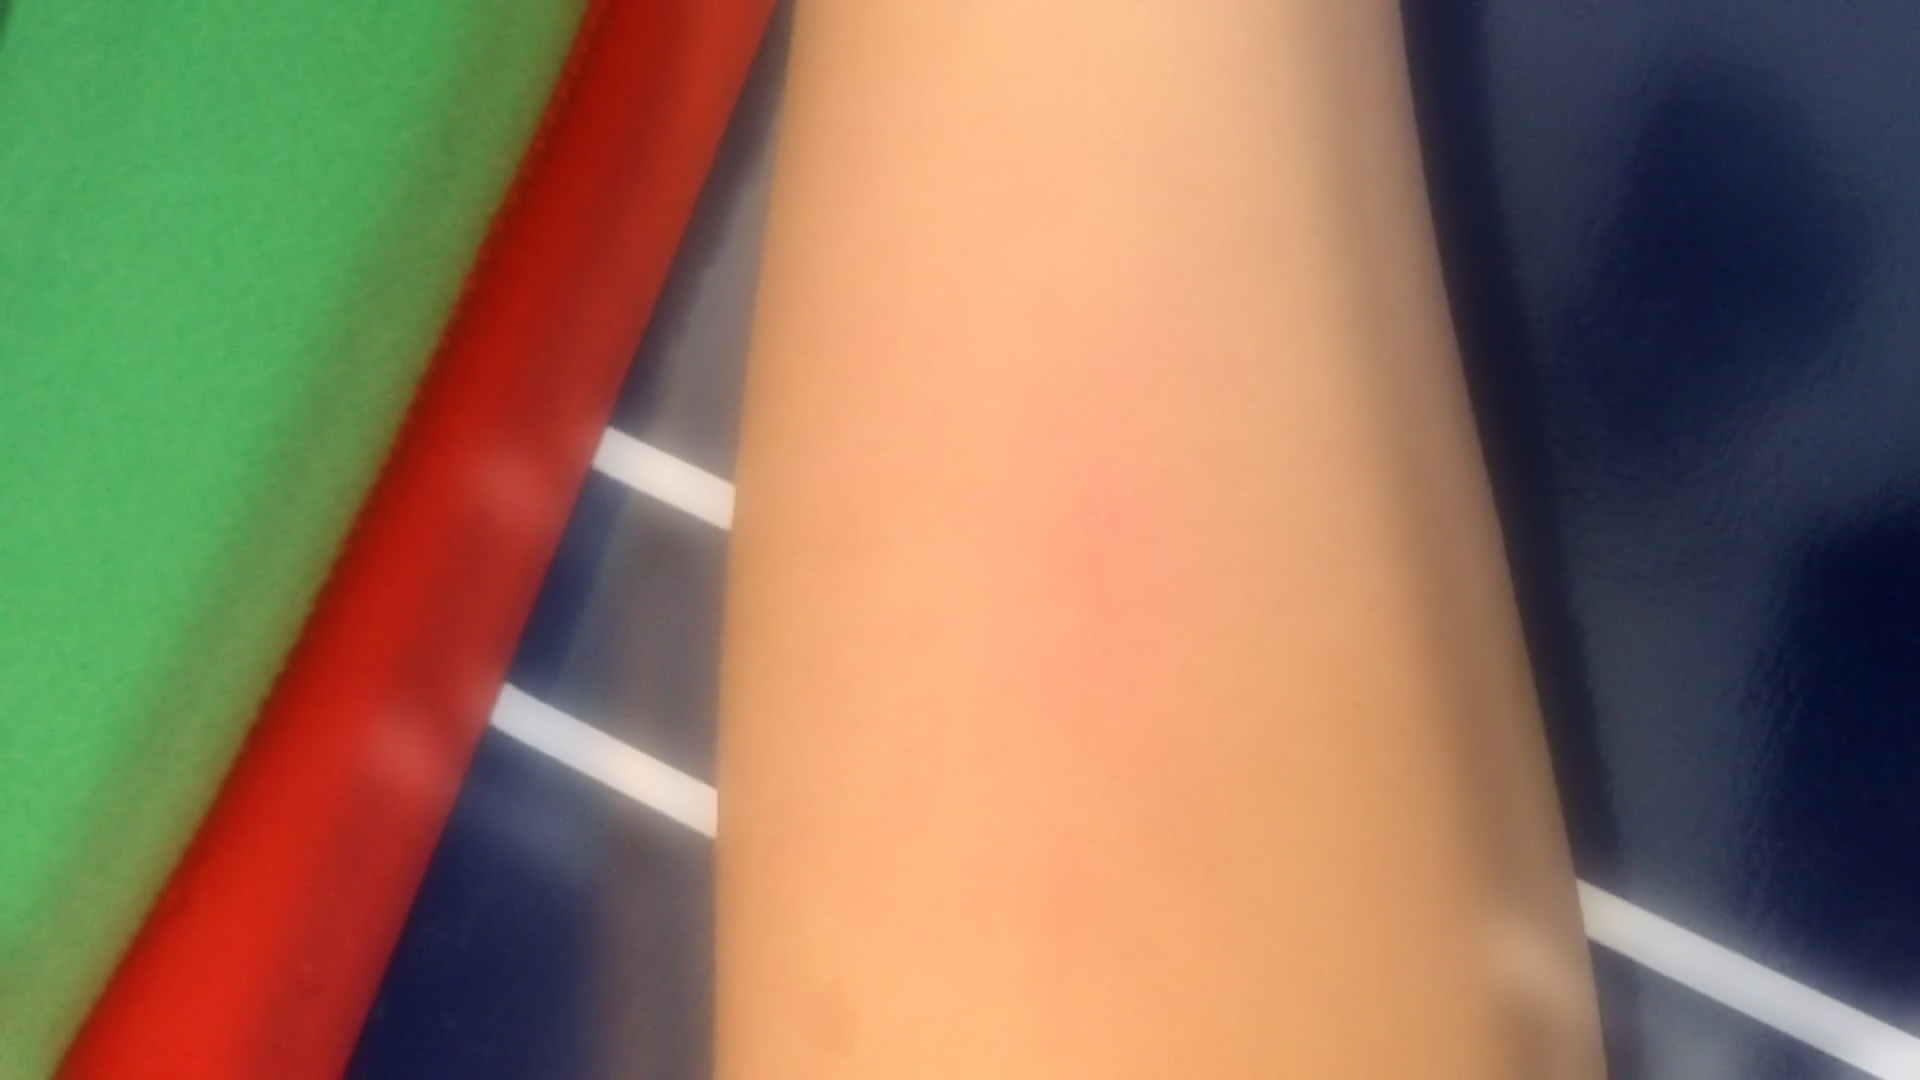
\includegraphics[scale=0.08]{img/eulerian/test/handc6}
  \label{fig:sub2}
\end{subfigure}
\caption{Differences of hand2 at frames sequences}
\label{fig:test}
\end{figure}

Hands were held still on a stable surface and the position of the Smartphone or camera was fixed during the recording. The results reveal periodic patterns in the frequency range after the Eulerian Video Magnification, that are caused by some subtle movements of the hands, which could not be held absolutely. This conclusion is strongly supported by the experiment shown in Figure 6.1. The pulse-related color changes are very difficult to visualize even under ideal conditions that are not realistic in many scenarios.\\

In the last experiment, different legs were directly recorded in different background and light sources. Leg1 became lighter and differences between the normal areas and pressure ulcers areas are made more significantly. Espacially for the second leg, after Eulerian Video Magnification, the blood vessel showed in the image, and the shadow is darker. \\

What's more, one of the drawback of this method is that it is trying to amplify color changes regardless of their source. When using the high amounts of magnification, it will lead to magnifying noise and compression artifacts making stray colors appear where we did not intend them to. The magnification was clearer on the darker face as it was less obvious when colors were being added than in the lighter face. In future, it is important to modify the proposed method to reduce the processing time as well as noise and attempt to make this process fully automatic.\\

\section{Some Constraints of Eulerian Video Magnification}
Those above mentioned experiments resulted in a set of strict constraints, in order to verify whether the Eulerian Video Magnification approach could work well under the specified controlled conditions:
\begin{enumerate}
    \item The camera and the recorded finger must be fixed during video capture, to make sure the changes are subtle.
    \item Lighting conditions should be well controlled to avoid impact caused by shadows or some changes in the illumination of the scene.
    \item The frequency range has to set based on multiple testing, because different part of human begin has subtle differences in frequencies.
\end{enumerate}
Those constraints constitute many limitations that render the Eulerian Video Magnification method for untained medical staff and day-to-day not suitable. A stable controlled light that imitates daylight was used, with an additional possibility to add backlight. \\

Futhermore, the Eulerian Video Magnification approach is extremely sensitive to the slightest changes in the source video. That requires a high quality video that is recorded using a fixed camera position. In addition, even in a scenario when the hands are held still on a flat surface to keep it stable and the camera position is fixed, the slight muscle shakes in the hands still cause strong responses in the result after Eulerian Video Magnification. Even in the ideal controlled conditions, it was not possible to make sure patterns would be clearly related to the color variations caused by the blood, it is expected that the future works will improve the use of Eulerian Video Magnification.\\

\section{Sensitivity to noise}

To extract as many information from the video as possible, this requires a high quality video discribed above, i.e. in an enough bright environment, to produce as minimal noise as possible. However, Eulerian Video Magnification still can amplify signals, which have smaller magnitude variations than the noise inherent in the video.\\

Assume that the noise is zero mean and equally distributed over the whole image. With suitable spatial low pass filters, the subtle signals will be enhanced. Compute the sum $\bar{x}$ of $N$ pixels as $\bar{x}=N\bar{x_{0}}$, where $x_{0}$ is the signal, and the sum of noise
power $\sigma ^{2}$ over $N$ pixel values as $\sigma ^{2}=N\sigma_{0} ^{2}$, where $\sigma_{0} ^{2}$ is the average noise power of a pixel,
we can increase the signal to noise ratio as\\
\begin{displaymath}
\frac{\bar{x}}{\sigma }=\frac{N\bar{x_{0}}}{\sqrt{N\sigma _{0}^{2}}}=\sqrt{N}\frac{\bar{x_{0}}}{\sigma_{0} }
\end{displaymath}

The ratio increases with the square root of the number of pixels taken.
As the number of pixels is proportional to the size of the area, which is $N\infty r$, over which the filtering is made, assuming that the bigger one is the area of averaging, the greater one is the signal to noise ratio.\\

Based on equation, it is estimated the area size that needs to be filtered, to reveal the signal at a certain noise power level. Figure 6.1 shows the importance of the proper spatial pooling.

 \begin{figure}
\centering
\begin{subfigure}{.5\textwidth}
  \centering
  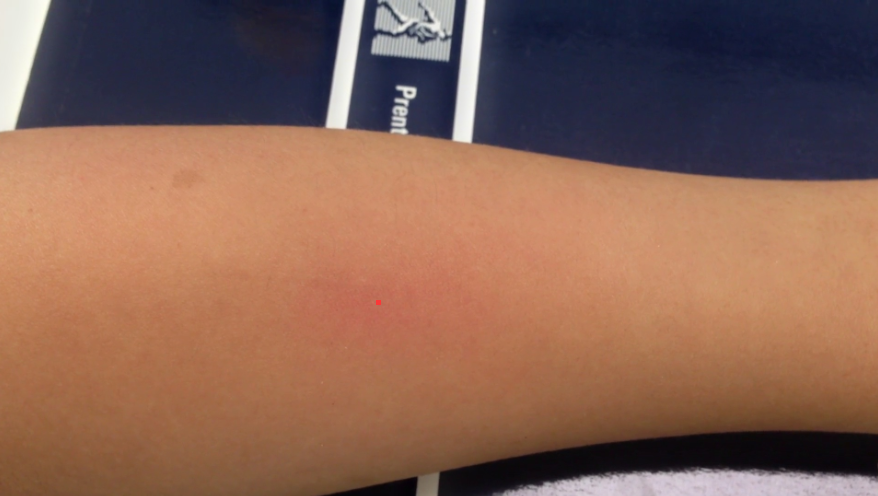
\includegraphics[scale=0.26]{img/noisepos}
  \caption{Original Frame without noise}
  \label{fig:sub1}
\end{subfigure}%
\begin{subfigure}{.5\textwidth}
  \centering
  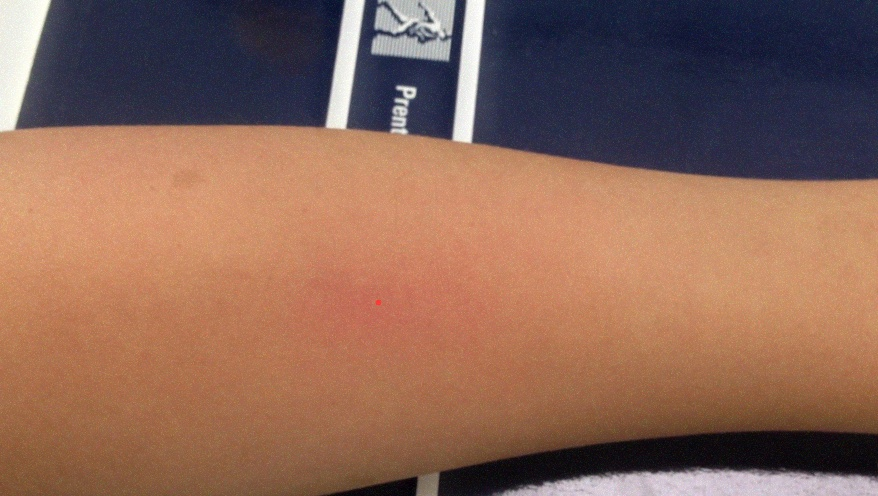
\includegraphics[scale=0.26]{img/noise}
  \caption{Original Frame with noise}
  \label{fig:sub2}
\end{subfigure}
\begin{subfigure}{.45\textwidth}
  \centering
  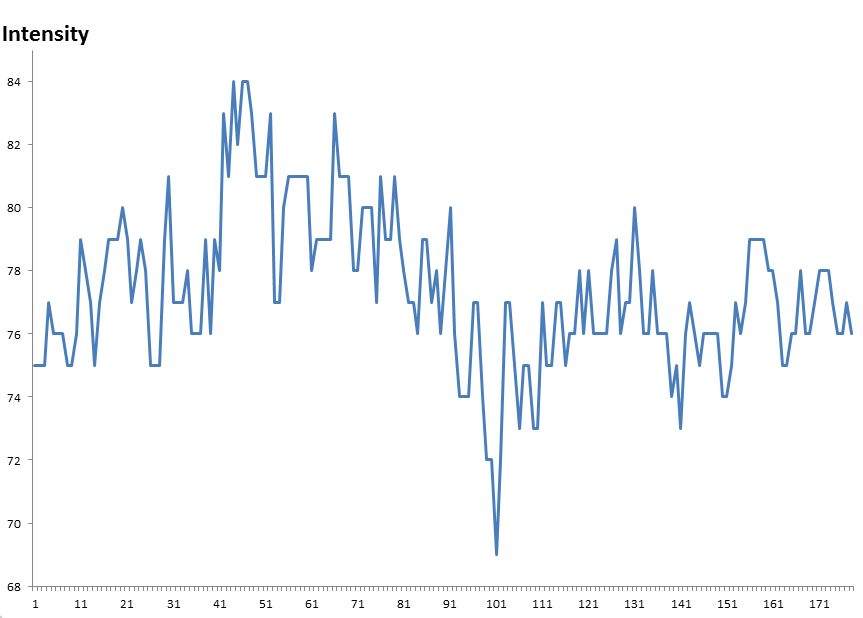
\includegraphics[scale=0.23]{img/intense}
  \caption{Insufficient Spaitial Pooling}
  \label{fig:sub2}%
\end{subfigure}
\begin{subfigure}{.5\textwidth}
  \centering
  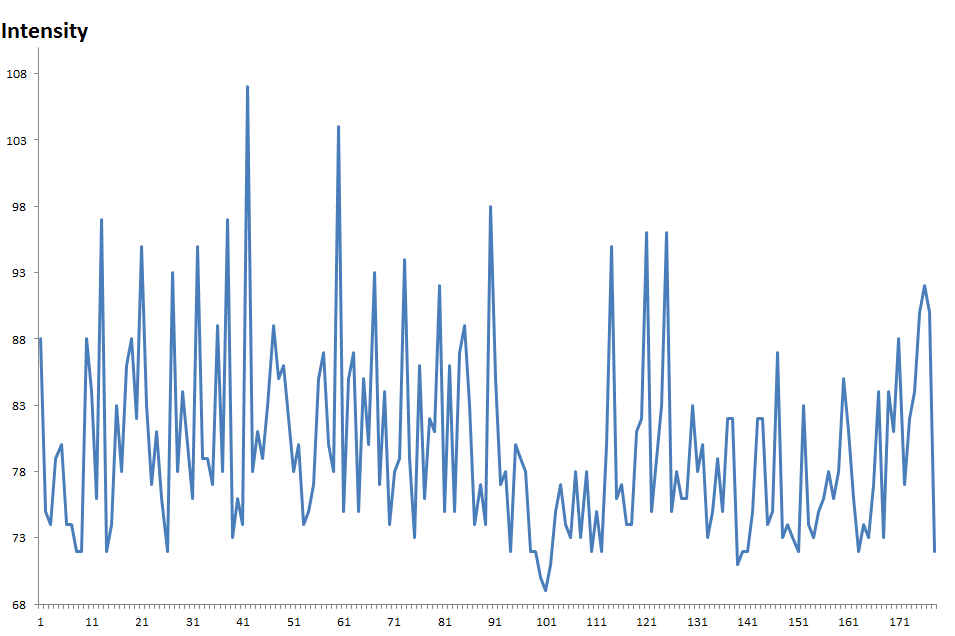
\includegraphics[scale=0.23]{img/intense2}
  \caption{Sufficient Spaitial Pooling}
  \label{fig:sub2}
\end{subfigure}
\caption{The importance of proper spatial pooling.}
\label{fig:test}
\end{figure}
\newpage
As Figure 6.2 shows, (b) shows a frame from a video on which Eulerian Colour Magnification was performed with $\sigma = 0.1$ pixel noise added. (c) and (d) show intensity traces over time, for the pixel on (a) and (b) marked blue. (c) shows
the trace obtained when the (noisy) sequence is processed with the same spatial filter used
to process the original face sequence. In this trace the pulse signal is not visible. (d) shows
the trace when using a filter with the filter size estimated. 